\documentclass[letterpaper,12pt]{report}

%\setlength{\parindent}{2em} %\setlength{\parskip}{1ex}
%\addtolength{\textheight}{24mm} \addtolength{\textwidth}{32mm}
%\addtolength{\topmargin}{-14mm} \addtolength{\oddsidemargin}{-30mm}
%\addtolength{\evensidemargin}{-30mm}
\usepackage{graphicx} % more modern
\usepackage{subfigure}
\usepackage{hyperref}
\usepackage{tikz}
\usepackage{amsmath}
\usepackage{amsthm}
\usepackage{latexsym}
\usepackage{amsfonts}
\usepackage{amssymb}
\usepackage{graphicx}
\usepackage{setspace}
\usepackage{graphics}
\usepackage{lscape}
\usepackage{times}
\usepackage{pgf}
\usepackage{algorithm}
\usepackage{algpseudocode}
\usepackage{theorem}
\usepackage{tikz}

\usetikzlibrary{shapes,arrows,automata}

% styles for flowcharts
\tikzstyle{decision} = [diamond, draw, fill=blue!20,text width=4.5em, text badly centered, node distance=3cm, inner sep=0pt]
\tikzstyle{block} = [rectangle, draw, fill=blue!20,text width=5em, text centered, rounded corners, minimum height=3.5em]
\tikzstyle{line} = [draw, -latex']
\tikzstyle{block2} = [rectangle, draw, fill=blue!32,text width=5em, text centered, rounded corners, node distance=4cm, minimum height=2.5em]
\tikzstyle{cloud} = [draw, ellipse,fill=red!20, text width=5em,text centered,node distance=2cm,minimum height=2em]
\tikzstyle{block3} = [rectangle, draw, fill=blue!20,text width=5em, text centered, rounded corners, node distance=3.5cm, minimum height=2.5em]

\begin{document}
\doublespacing

\pagenumbering{roman}
\tableofcontents
\cleardoublepage
\listoffigures
\cleardoublepage
\listoftables
\cleardoublepage

\begin{abstract}
Although temporal data provides critical context for many real-world reasoning tasks, incorporating the temporal dimension into an analysis can present methodological challenges.  Traditional methods from statistics are limited in their ability to process large-scale secondary data sources, and data mining approaches have primarily focused on static data sets.  However, few real-world data sets are by nature static, or are designed to measure stationary phenomena; rather, they are dynamic.

Using electronic health record (EHR) data as a case study, I develop a new exploratory analysis method to facilitate meaningful use of abundant temporal EHR data and provide insights into chronic disease progression.  Semiparametric clustering is a framework that uses parametric models to provide a principled way to summarize, `\emph{abstract}', variable length temporal sequences for comparison, and a nonparametric clustering step to reveal inherent groups.  To model the dynamics of chronic conditions that may progress over a period of years, I extend current applications of the semiparametric clustering to learn characteristic groups of patients from EHR repositories with temporal sequences that are variable length, subject to a variety of sampling schemes, and contain data that is not missing at random.

Specifically, continuous-time models are used to more directly represent time, and address the limitations of discrete-time abstraction. Also, current applications of semiparametric clustering require specifying $k$, the number clusters, $a$ $priori$. I propose pairing model-based abstraction with a nonparametric Bayesian clustering method that allows $k$ to be expressed as a function of the size and complexity of the patient population.

%To model chronic disease dynamics, which may evolve slowly, over years, we extend current applications of the semiparametric clustering framework~\cite{JebSonTha07a} for learning patient and population level disease characteristics from arbitrarily sampled longitudinal patient data.  Specifically, we use parametric models based on continuous time Markov models paired with nonparmetric Bayesian clustering and we show results for two distinct data sets.

 Clustering performance is evaluated on two clinical data sets.  Using lab data from hepatitis patients, I show a 20\% relative improvement on a benchmark for grouping patients by fibrosis score.  The second data set contains encounter data, indicating physician ordered glucose test for hospitalized patients.  Although there is no gold-standard for comparison, my method can detect recognizable differences among discovered groups that can be visualized, and produces good clusters based on intrinsic quality metrics.


%Although the discrete-time assumptions these parametric models make are an useful simplifying assumption for many data sets, they can be problematic when data is not missing at random.  Also, a key limitation of many clustering methods is that the number of clusters must be indicated $a priori$. For patient data, where the number of groups can vary based on the sample a more flexible approach that allows $k$ to be expressed as a function of the size and complexity of the data is more desirable.


\end{abstract}


\newpage
\pagenumbering{arabic}

\chapter{Introduction}
\label{ch:intro}
\chapter{Introduction}
\label{ch:intro}

\section{Motivation}
The availability of clinical data repositories presents new opportunities for improving health care quality and reducing costs.  However, the secondary function of these data sources as research tools presents challenges for longitudinal data analysis.  To facilitate the meaningful use of abundant temporal EHR data, I develop a probabilistic \emph{temporal clustering method} that can assist in the preprocessing, exploration, and discovery of new knowledge from these noisy, heterogenous, fragmented data collections.

Clustering is a pervasive and natural human activity that affects knowledge representation and discovery~\cite{Guyon}.  Typically, we use it to group similar objects together, and establish criteria that are useful for their definition.  Computational clustering algorithms can help reveal inherent group structures, or clusters, among observations without requiring the use of class labels for learning.  For large data sets that are high dimensional, and where the distinguishing characteristics for establishing class boundaries are unknown, this application is particularly useful for exploratory analysis, and can enable a systematic examination of a data set.  In addition, clustering can be used as a preprocessing step with the aim of enriching the quality of a data sample by filtering noisy or less informative examples.

For phenomena that evolve over time, the magnitude and direction of changes, and when changes occur can provide critical context for reasoning.  Not only are there resource issues associated with the increased size of a temporal data set, but modeling choices related to the representation of temporal granularity and sequential dependencies must be considered.  Also, secondary sources of temporal data are especially challenging.  Many contain measurement sequences that are irregular in length, and subject to a variety of sampling schemes, resulting in irregular time intervals between observations, and data that is not missing at random.

%Although temporal data provides critical context for many real-world reasoning tasks, incorporating the temporal dimension into an analysis can present methodological challenges.  Traditional methods from statistics are limited in their ability to scale to data sets with thousands of time points and noisy secondary data sources, and data mining approaches have primarily focused on static data sets.  However, few real-world data sets are by nature static, or are designed to measure stationary phenomena; rather, they are dynamic and contain information about values that change over time.

 %A variety of learning algorithms, have been developed to address the limitations of traditional approaches for modeling real-world time series sequences that are large-scale, subject to noise, and serve a secondary purpose as a research instrument.

 A variety of learning algorithms, have been developed to address the limitations of traditional approaches for modeling real-world time series sequences.  Regardless of the task, the first step involves \emph{abstraction}, a process of transforming the raw data in to a high-level representation that facilitates description and comparison among sequences, typically to retain only information which is relevant for a particular purpose.  Of the main methods, model-based abstraction is the only technique that provides a direct correspondence with the description of the underlying data generating process, and provides a principled way to transform variable length observation sequences into a uniform number of descriptive parameters, facilitating its use for additional analysis and interpretation.

To cluster temporal sequences, the \emph{semiparametric clustering} framework described by Jebara et al.~\cite{Jebara} pairs structural and parametric assumptions such as Markov properties for discrete-time abstraction, with nonparametric spectral methods to cluster the abstractions, priors of the model parameters for each sequence, instead of the raw time series sequences.  In addition to demonstrating state-of-the-art performance on a variety of temporal data sets, their experiments show clear benefits of hybrid methods instead of fully parametric, or fully non-parametric methods.

In this thesis, I extend the semiparametric clustering framework to address common challenges to modeling temporal EHR data.  Although discrete-time assumptions provide useful simplifying assumptions for modeling many temporal data sets, Bayesian networks~\cite{Dean89} and their variants are less appropriate for processes that that are observed by arbitrary sampling schemes, such as self-selection, or that may evolve on a non-linear trajectory.  Also, spectral clustering methods assume the number of clusters, $k$, is fixed.  For patient data, where the number of groups can vary based on the sample, a more flexible approach that allows $k$ to be expressed as a function of the size and complexity of the data is more desirable.

To more directly represent patient data related to chronic disease progression, the specific models I develop for abstraction are based on finite state \emph{continuous-time (CT) Markov processes}.    Specifically, I use CT Bayesian networks (CTBNs)~\cite{Nodelman02}, incorporating theoretical aspects of multi-state Markov models (MSMs)~\cite{Jackson10} that are used form disease modeling in epidemiology and biostatistics.  MSMs share the same theoretical foundations as CTBNs and are based on domain knowledge that many chronic diseases have a natural interpretation that results in a staged progression of disease related states. In addition, I extend applications of clustering to the nonparametric Bayesian setting, allowing for a clustering model that is more expressive, and no longer requires that $k$ is established by a heuristic $a$ $priori$.

%When there are no natural time slices, CT Bayesian networks (DBNs)~\cite{Nodelman02} more directly reflect sequential dependencies, and in contrast to discrete-time models do not force the representation of missing data.  Notably, a class of DBNs known as multi-state Markov models (MSMs)~\cite{Jackson10} in biostatistics.  Traditionally, MSMs are used to examine population based disease dynamics from smaller longitudional data sets.  They have not been applied for comparisons among patients, or as the basis for temporal clustering.


%To more directly represent time, I extend temporal abstraction to an class of continuous-time Bayesian networks (CTBNs)~\cite{Nodelman02}, which share with multi-state Markov models (MSMs)~\cite{Jackson10}.  MSMs are used by epidemiologists to model population disease dynamics in biostatistics and share a foundation in finite state \emph{continuous-time (CT) Markov processes}.    Specifically, In addition, I extend applications of clustering to the nonparametric Bayesian setting, allowing for a clustering model that is more expressive and no longer requires that $k$ is known $a priori$.

%Traditionally, MSMs are used to examine population based disease dynamics from smaller longitudional data sets.  They have not been applied for comparisons among patients, or as the basis for temporal clustering.

%The experiments I conduct aims to cluster patients of similar health status together in the same cluster, and to represent distinct qualitative groups in separate clusters, with each cluster of maximal size.

%Although this framework is appropriate for many types of data sets, the types of models used for abstraction, Bayesian networks~\cite{Dean89} and their variants, make discrete-time assumptions that are less appropriate for data that is not missing at random, and EHR data can be subject to arbitrary sampling schemes, and patient self-selection is common.  Also, spectral clustering has been the consistent choice for the nonparametric clustering step of the semiparametric framework, and requires that the number of clusters, $k$, is fixed.  For patient data, where the number of groups can vary based on the sample a more flexible approach that allows $k$ to be expressed as a function of the size and complexity of the data is more desirable.

%To more directly represent time, the specific models I develop for temporal abstraction are based on finite state \emph{continuous-time (CT) Markov processes}.    Specifically, I extend temporal abstraction to an class of CT Bayesian networks (DBNs)~\cite{Nodelman02} known as multi-state Markov models (MSMs)~\cite{Jackson10} in biostatistics.  Traditionally, MSMs are used to examine population based disease dynamics from smaller longitudional data sets.  They have not been applied for comparisons among patients, or as the basis for temporal clustering.

%Rather than use the sequences of values directly, we build probabilistic models, abstractions, of these sequences using continuous-time models.

%In this thesis, using longitudinal data extracted from EHRs to model chronic dynamics, I extend the framework of semiparametric temporal clustering to address the some of the challenges posed by clinical data, and describe a new exploratory analysis method for learning patient and population level chronic disease dynamics.  Specifically, I extend the framework of semiparametric clustering to continuous-time Bayesian networks (CTBNs)~\cite{Nodelman02} for model-based abstraction.  When there are no natural time slices, CTBNs more directly reflect sequential dependencies, and in contrast to discrete-time models do not force the representation of missing data. In addition, I extend applications of clustering to the nonparametric Bayesian setting, allowing for a clustering model that is more expressive and no longer requires that $k$ is known $a priori$.



%Clinically significant work applying exploratory techniques to clinical data has been demonstrated~\cite{Saria09, Marlin12}, but it has focused on monitoring patients in the critical care setting, where data is sampled at a high frequency.  In contrast, modeling the evolution of a patient's chronic disease trajectory may require data that has been sampled for a duration of months or years, and in EHR collections, the assumption that data is missing at random is less likely to be true.


%The key benefits of this abstraction approach is a principled way to represent variable length raw data as a uniform length vector.  However, they require that time is discretized, and represented as series of steps that are equal to the smallest time granularity in any observed sequence.  Although discrete-time models are suitable in many cases, there are two key limitations that  relevant to EHR data. First, if the underlying health phenomena progresses in individuals at different rates, one granularity must be used to express time steps for the entire system. Second, when data is unavailable, intervening time slices must still be represented.

%When there are no natural time slices, continuous-time BNs (CTBNs) (Nodelman et al., 2003) can be used to more directly reflect sequential dependencies, and avoid discretizing the time intervals.  Notably, a domain specific instance of CTBNs, Multi-state models (MSMs), are used in epidemiology and biostatistics as Multi-state models (MSMs) for modeling population level disease dynamics.  Our work builds upon these theoretical foundations in CTBNs and MSMs to develop a continuous-time abstraction method for longitudinal EHR data.

Lastly, the reasons described above motivate this work but it is important to note the following.  Although unsupervised learning methods have many successful applications, one substantial obstacle to their practical adoption is the difficulty of interpreting results.  Many clustering metrics are based on a mathematical interpretation of clustering as a partitioning problem that is independent of problem context.  However, it is clear the purpose of clustering, and the context of its end-use are crucial aspects to consider when determine if results are useful or meaningful~\cite{Guyon}. For this reason, I evaluate my method using established validation metrics from the literature, and develop visualization tools to help communicate and examine the clinical context and significance of my work.

%Bayesian Nonparametrics is a rapidly growing subfield of statistics and machine learning that provides a framework for creating complex statistical models that are both expressive and tractable.

%some beneficial structural and parametric assumptions such as Markov properties and hidden state variables which are useful for clustering

%For the purpose of inference, the goal of temporal abstraction is to provide a concise, high-level description of a sequential process that facilitates description and comparison among sequences, while simultaneously preserving the information contained in the raw data.

%can provide insight into the nature of dynamic processes that are not well understood.  For scientific inquiry, they help automate the systematic examination of an entire collection, and can be used to generate new and important hypotheses that may not have been identified by a human expert.   Also, they can be used as a preprocessing step with the aim of enriching the quality of a data sample by filtering noisy or less informative examples.

%Although unsupervised learning methods are the focus of considerable work in machine learning, extending their use for sequential data remains challenging.

%Despite noted limitations by researchers, clustering methods have been used effectively as an exploratory analysis step for driving scientific inquiry towards more targeted hypotheses, or as a preprocessing step to enrich the quality of a data sample by filtering noisy or less informative examples.  As databases evolve over time, growing in number, size and scale, and more resources are available to efficiently processing data, methods for temporal data modeling and analysis are of increasing importance.  %In the context of inquiry,  exploratory methods methods can enable exploratory analysis, and be used to generate new and important hypotheses that may not have been identified by a human expert.
%Also, they help automate the systematic examination of an entire collection instead of a preselected sample, reducing the impact of experimenter and other biases that have been associated with false findings~\cite{Ioannidis05}, and can be used to generate new and important hypotheses that may not have been identified by a human expert.

%temporal analysis
%Time provides critical context for many real-world reasoning tasks and temporal clustering can provide insight into the nature of dynamic processes that are not well understood.  For scientific inquiry, they help automate the systematic examination of an entire collection, and can be used to generate new and important hypotheses that may not have been identified by a human expert.   Also, they can be used as a preprocessing step with the aim of enriching the quality of a data sample by filtering noisy or less informative examples.

%Existing data mining approaches have demonstrated their ability to reveal unseen patterns and summarize data in meaningful ways, but they have primarily focused on static data sets, where the assumption that data is independently drawn and distributed (i.d.d.) is less problematic.  However, few real-world data sets are by nature static, or are designed to measure stationary phenomena; rather, they are dynamic.   Not only is the i.i.d. assumption more problematic for temporal learning, real-world data sets often provide measurement sequences that are irregular in length, arbitrarily sampled and may contain data that is not missing at random (MAR).  Together these collective conditions present methodological callenges for existing data mining methods, and more traditional statistical methods.

%temporal clsutering
%Regardless of the temporal learning method, abstraction is almost always
%Abstraction is the process by transforming a concept or an observable phenomenon in to a more succinct form, typically to retain only information which is relevant for a particular purpose. For the purpose of inference, the goal of temporal abstraction is to provide a concise, high-level description of a sequential process that facilitates description and comparison among sequences, while simultaneously preserving the information contained in the raw data.

%A range of methods have beed developed to address the limitations of traditional analysis methods for modeling time.  They can be broadly categorized as subsequence, feature and model based, and primarily aim to transform the raw data into a more concise, high-level description of a sequential process that facilitates description and comparison among sequences.   In contrast to subsequence based methods, model based approaches can be used to abstract whole sequences, and facilitate the comparison of uneven length sequences.  Also, they do not require the overhead of a feature engineering process, which aims to extract information in order to characterize the shapes that correspond with change along the temporal trajectory.

%What has been developed in the data mining and machine learning community for temporal modeling are two main approaches: feature engineering and model based abstraction.  There are many successful feature based temporal mining algorithms, but they are task specific.  Feature-based approaches extract information in order to characterize the shapes that correspond with change along the duration of the temporal trajectory.  Also, they don't have a direct correspondence with the description of the phenomena or underlying process more generally.

%Bayesian Nonparametrics is a rapidly growing subfield of statistics and machine learning that provides a framework for creating complex statistical models that are both expressive and tractable

\section{Contributions}

The central contribution of this thesis is to introduce a new probabilistic learning method for the exploratory analysis of non-canonical time series data.  Although, clinically significant work applying exploratory techniques to clinical data has been demonstrated~\cite{Marlin12,Saria09}, it has focused on monitoring patients in the critical care setting, where data is sampled at a high frequency and the clinical concerns are more immediate.  In contrast, chronic disease progression can take months or years to manifest, and longer-term trends can have increased importance.

%In contrast, modeling the evolution of a patient's chronic disease trajectory may require data that has been sampled for a duration of months or years, and the assumption that data is missing at random is less likely to be true.

%Using electronic medical data as a case study, I develop a method for modeling patient and population chronic disease dynamics that can be used to model data the reflects variable durations, that is subject to a variety of sampling schemes.  Specifically, I extend the framework of semiparametric temporal clustering~\cite{Jebara} to continuous-time abstraction and nonparametric Bayesian clustering.

%I evaluate the performance of this approach on two clinical data sets.  Using lab test data for hepatitis C patients and aiming to cluster patients by liver fibrosis stage, my method shows over a 20\% relative improvement over benchmark performance.  The second data set contains encounter data, indicating physician ordered glucose test for hospitalized patients.  Although there is no gold standard for comparison, my method can detect recognizable differences among discovered groups that can be visualized, and produces good clusters based on intrinsic quality metrics.


%Specifically, I present \emph{new extensions to the semi-parametric framework}.Using electronic medical data related to chronic conditions as a case study, I focus developing a new method for clustering patient-level electronic health record (EHR) data that is collected for variable durations, and sampling schemes.  There is an existing body of work modeling temporal patient data in the critical care environment, where a high sampling frequency signal is provided by physiological measurements~\cite{Russel08,Saria10,Marlin12}.   Although these methods are innovative and have shown benefits for clinical care, the techniques do not easily translate to electronic health record (EHR) data that is subject to longer durations, such as months or years, and the noise and incompleteness associated with secondary data sources.

% When used as data sets for research, secondary data sources, such as electronic health record data, transaction data bases, social media and others, pose methodological challenges.  That is, they may provide a signal, but one that is muddled with noise, and they may be incomplete, forcing traditional methods to make assumptions about missing data values that may not be true.




%Patient level observational data that is collected over time is commonly referred to as panel data in econometrics and statistics, and longitudinal data in biostatistics.  The main distinction of my application from what is typically the subject of study in these fields is the secondary nature of the data set, and the size.  The traditional methods for longitudinal analysis of patients are designed to model far fewer time points, require uniform length sequences, and data is collected for the purpose of the study.

More specifically, the contributions of this thesis are:
\begin{itemize}
  \item I introduce a temporal clustering method designed to utilize the temporal data that serves a secondary purpose as a research instrument.
  \item I describe how continuous-time model based abstraction can be used to provide a principled approach to regularizing time series that are variable in length, subject to arbitrary sampling schemes, and reflect irregular intervals.
  \item I develop a continuous-time abstraction method for clinical data that more directly models observations, and incorporates theoretical aspects of multi-state Markov models that are used in biostatistics for survival analysis.
  \item I extend the semiparametric framework to the nonparametric Bayesian setting.  This no longer requires that $k$ is fixed, or a required parameter for clustering.
  \item I demonstrate that my clustering approach can produce meaningful clusters from noisy, incomplete patient data and evaluate results on intrinsic and extrinsic validation methods.
  \item I discuss the clinical significance of clustering results, and what findings have a potential translation to practice.
  \item I show that my clustering approach improves on state-of-the-art performance by comparison with a benchmark system on gold-standard results.
  \item I compare the performance of nonparametric Bayesian clustering with spectral methods for clustering patient models.
  \item I facilitate the interpretation of model-based clustering results by normalizing cluster-level characteristics and visually compare group signatures in terms of ``instantaneous risk''.
\end{itemize}



\section{Overview}
This work extends applications of semiparametric clustering methods for temporal data and describes two experiments using clinical data sets to evaluate performance.

A background on temporal analysis methods, including semiparametric clustering is discussed in more detail in Chapter~\ref{ch:temporal_dynamics}.

Related work that this thesis builds upon in continuous-time representations, biostatistics, and Bayesian clustering is detailed in Chapter~\ref{ch:related}.


%Using electronic health record data from patients with or at risk of chronic disease as a case study, we develop a new approach for learning temporal dynamics from a secondary data source that contains variable length sequences, is measured at irregular time intervals, subject to arbitrary sampling schemes, and subject to incompleteness

%Related work that this thesis builds upon in continuous-time representations, epidemiology, and Bayesian clustering is detailed in Chapter~\ref{ch:related}.

 I describe the variety of methods for temporal abstraction in Chapter~\ref{ch:abstraction}.  Their relationship to clustering, and a comparison of clustering methods are provided in Chapter~\ref{ch:clustering}.

 My novel contributions begin in Chapter~\ref{ch:new}, where I discuss continuous-time representations for patient level disease modeling, the integration of nonparametric Bayesian clustering.

 I evaluate the performance of this new approach to semi-parametric clustering on two data patient-level data sets, including a hepatitis and glucose data sets in Chapter~\ref{ch:expts}.

Finally, a summary of this work, the key conclusions and next steps appear in Chapter~\ref{ch:conclusions}.

\section{Publications}
The work described in this thesis has appeared in several publications:
\begin{itemize}
  \item Tamang S and Parsons S. (2013a). Semiparametric Clustering Methods for Modeling Chronic Disease Dynamics. \emph{In Proceedings of the International Conference on Machine Learning, Workshop on the Role of Machine Learning in Transforming Healthcare.}
  \item Tamang S and Parsons S. (2013b).  Unsupervised Modeling of Patient-level Disease Dynamics. \emph{In Proceedings of the Association for the Advancement of Artificial Intelligence Spring Symposium, Workshop on Data Driven Wellness.}
  \item Tamang S and Parsons S. (2011). Using semi-parametric clustering applied to EHR time series data. \emph{In Proceedings of the Knowledge Discovery and Data Mining, Workshop on Data Mining for Medicine and Healthcare.}
\end{itemize}

In Chapter~\ref{ch:related}, I describe preliminary work for this thesis that appears in Tamang and Parsons (2011) and demonstrates the appropriateness of semiparametric clustering methods for EHR data by comparing the framework with alternative approaches.  I extend semiparametric clustering to continuous-time model abstraction and the nonparametric Bayesian setting in Tamang and Parsons (2013a; 2013b) and this material appears in Chapters ~\ref{ch:new} and ~\ref{ch:expts}.






%motivation
%contribution
%%%supervised and unsupervised learning
%%%temporal mining
%%%Electronic Health Records
%%%Disease Progression Models

\chapter{Temporal Modeling}
\label{ch:temporal_dynamics}
\chapter{Background}
\label{ch:temporal_dynamics}

Time is undoubtedly one of the most mysterious concepts.  We may learn to `tell time', but our understanding is so natural, and empirically enforced that we never need to explicitly be be told or reminded of its basic qualities.  However, when analyzed more critically, or scientifically, time is paradoxical and its nature, construction and impact continues to occupy the minds of great thinkers.

Two critical assumptions are made by automated reasoning methods. First, a underlying characteristic of unidirectionality, that defines time as an infinite, forward moving trajectory.  Secondly, that information about the past can be propagated along this temporal trajectory, or a quality of persistence.  These two assumptions are perhaps the most basic, and are consistent with an enormous amount of evidence that can be observed in both our internal and external environments.

Methods for modeling temporal data vary most dramatically not in a rejection of these basic assumptions, but rather the simplifying assumptions that facilitate analysis and are used to structure and summarize raw time series values.  Many are known to be false, for example representing a temporal process by modeling one snapshot, but are either required for any analysis at all, or present a limited effect on results.

\section{What are the Questions to Ask?}
When little prior knowledge about group structure is known and a collection of observations is too large for a human to peruse, unsupervised-learning algorithms, also known as unsupervised classification, can be useful.  To this end, we have developed a clustering method for longitudinal patient data that more easily extends to new data sets, and in contrast to discrete time approaches, is more appropriate for the preprocessing and exploratory analysis of incomplete, irregular observation sequences that are common to patient data found in electronic health records.

Clustering is a pervasive and natural human activity that us used for a variety of tasks. Typically, we use it to group similar objects together so that we can assign characteristics that are useful for their definition.   At the minimal level, automated clustering can be viewed at preprocessing with the goal of improving the performance of a system.  For example, in a collection of patients with a potentially lethal disease only diagnosed using an invasive procedure, clustering can help to determine those patients of minimal risk.  A consequent processing step can focus on the set of patients more likely to develop a terminal condition.

In the context of exploratory data analysis, clustering techniques are applied to data with the aim of discovering underlying patterns that can be used to generate new hypotheses for more targeted data analysis.  However, the interpretation of cluster goodness can be problematic.  Even with a gold standard for evaluation performance, it is important to note that within a specific domain of application, there can be opposing views that are not resolvable.  For example, in biology there can be very diverse views on the classification of the same organism~\cite{pmid20500846,pmid23209778}.

\section{Time as Critical Context}
Sequential data can exist in the form of word order in a sentence, or it can exist in a more explicit temporal form that is generated by a process.  This work focuses specifically on temporal data, which are a special form of sequential data that are typically measured uniformly, and often referred to as `time series', but may reflect variable time granularities and other irregularities that required a modeling process to account for more uncertainly.

\subsection{The Flow of Time}
The philosophy of space and time and whether it exist independently from each other, is a question of the most importance, but beyond the scope of this thesis.  For the purpose of this work, we assume that time is a unidirectional flow and continuous in nature.  We also assume that the dynamic processes can be represented at specific instances using a temporal marker.  For this reason, we can measure the change of a process with respect to time by observing the differences between any two time markers, or points, on a temporal trajectory.

In this work, we do not attempt to theorize about the underlying nature of time.  However, we do make a case for a more accurate representation to model temporal dynamics that have direct relevance to important data analysis problems.  That is, for processes monitored at fixed intervals, the discretization of time into a vector of uniform length fragments, is an appropriate modeling assumption.  Although no one would argue that time is discrete, when observations are collected in high-frequency settings, or continually monitored at regular intervals it presents benefits.  However, this is not appropriate in the case in data sources that evolve in continuous time, subject to variable sampling schemes and incomplete.


\section{Semiparametric Temporal Clustering}
Regardless of the temporal mining task, the first step of an algorithm is to transform, or abstract, the raw data into a more concise representation, preserving as much of the information contained in the original sequence as possible.  \emph{Semiparametric temporal clustering} makes useful parametric assumptions to approximate temporal data and regularize sequences for input to a clustering step.  The temporal abstractions, abstractions of the raw time-series, function as input to a nonparametric clustering algorithm, which seeking to reveal underlying structure and be more agnostic about properties of the resulting clusters.

\begin{figure}[t]
\vskip 0.2in
\begin{center}
\centerline{\includegraphics[width=\columnwidth]{fig/semipoverview.jpg}}
\caption{An Overview of Semiparametric Clustering}
\label{semipoverview}
\end{center}
\vskip -0.2in
\end{figure}

Figure~\ref{semipoverview} shows an overview of the semiparametric temporal clustering framework. The first step entails temporal abstraction using a parametric model to transform a set of raw time series for $N$ observations, $X_1, X_1,...,X_N$, into a more manageable form for traditional multivariate clustering algorithms. It entails learning each patients model-specific parameters, $Q_1, Q_2, ..., Q_N$, from the time series observations.

The second step is nonparametric clustering. Spectral methods are typically used in the semiparametric framework, which requires determining the number of clusters, $k$, in advance. In this work, we extend the
clustering component to the nonparametric Bayesian setting, allowing for the number of clusters to be expressed as a function of the sample size.

\subsection{Modeling Chronic Disease Dynamics}
One specific case for which discretization of the temporal trajectory into regular intervals has been known to contribute to error, is that of longitudinal data derived from monitoring disease phenomena and is why there are fewer applications of discrete-time Markov models in medicine~\cite{Jackson2011}.  SInce observations are typically documented only during hospital or physician visits, resulting in irregular time intervals.  Also, a patient's measurement sequence be short or can span over many years and the nature of the observation scheme (e.g., fixed, random or self-selected) can be unclear.

Despite these challenges, health services researchers generally agree that electronic health record (EHR) data provides many opportunities for new knowledge discovery, and there is tremendous potential for value beyond meaningful use.  The temporal dimension of indicter data provides critical context for diagnosis and prognosis of many patients suffering from chronic diseases.

Historically, following a cohort of individuals entailed the design of customized measurement tools to monitoring patients for a research study and explicit checkpoints for data collection.  Now, the number of human data artifacts is increasing, and each new datum has the potentially help to provide further clinical insights.  Conventional methods for temporal mining are not designed to accommodate for the type of noise incompleteness, and other features that are associated with modeling from patient records.  To provide a better understanding of dynamic changes that can occur during the course of a patient's disease trajectory, this work examines new semi-parametric clustering methods for temporal data.

Currently, when exploratory analysis is performed in electronic health records (EHRs ) it does not consist of a automated examination of possibilities and potential structures.  Rather, a domain expert will typically use prior knowledge to reason about distinctions within a population, and carefully select a sample or sub-population that they suspect may result in significantly different clinical or other outcomes.  These prior assumptions guide targeted research questions, and are more likely to result in findings~\cite{Ioannidis05}

\section{Modeling Challenges}
\subsection{Selecting the `Right' Granularity}
\subsection{Sampling and Aligning Temporal Data}


\chapter{Related Work}
\label{ch:related}
\chapter{Related Work}
\label{ch:related}

In this chapter I discuss work that this thesis builds upon.  Numerous approaches exist for approximating temporal data and in the first section I discuss work
\section{Model-based Clustering}
\label{ch:related}
For the task of temporal clustering, the use of Markov-based approaches to model time series has been shown to produce high performance results in several domains.  The beneficial parametric assumptions they make are used for abstracting temporal data to describe temporal dependencies.  Almost all existing model-based methods use a Markov chain, many with extensions for hidden states, to represent the temporal dynamics of observation sequence.  Among the various techniques that appear in the research literature on Markov-model abstraction, the key distinction is how the model parameters are used for clustering.

The most popular approach is to describe a time series dataset as generated by $K$-HMM components and identify $K$.  For example, we can describe a dynamic process using:
      $$f_{K}(O)=\sum_{k=1}^{K}f_{k}(O|\theta_{k})w_{k}$$
where,  $O$ is a time series, $w_{k}$ is a weight of the $k$th HMM and $f_{k}(O|\theta{k})$is the probability that the series was generated by the component model $f_{k}$ with parameters $\theta_{k}$.  To estimate $K$ many clustering approaches of this type impose additional parametric assumptions about cluster shape~\cite{Shah2009,Zeng2006,preprints429}.

In terms of nonparametric approaches that complement modelbased abstraction, spectral methods have been paired with HMM abstraction for \emph{semiparametric clustering}.   In this approach, models are embedded in that their parameters are used as input to the clustering step and it is sometimes referred to as clustering with embedded models.   Here, the model represents the time series in a concise and descriptive way, and provides a principled approach to handling variable length temporal sequences~\cite{Yin_Yang_2005,Jebara_07}.  

 The semiparametric framework for time series clustering was motivated by the ambition to apply high-performance clustering methods that allow the data miner to be agnostic about the structure of the resulting group.   Notably, using this approach to semi-parametric clustering Jebara et al.~\cite{Jebara_07} have clustered motion capture data and show better performance relative to clustering with mixtures of HMMs, and comparable to that which was achieved with supervised learning.  Further building on the general semi-parametric framework, and also using embedded HMMs with spectral clustering, Garcia et al.~\cite{GarciaHD09,Garcia2011} examine the impact of alternative similarity metrics to compare models derived from individual observations and their ability to create structured distance matrices that are consequently exploited by spectral methods.

An alternative nonparametric approach for clustering time-series has been described in recent work using Markov model abstraction.  Fruhwirth et al.~\cite{Pamminger_Fr_2010} pose the clustering task as estimating the priors for $K$ components of a Dirichlet distribution.  Similar work in sequential data is more prevalent, and since a Bayesian method is typically used to estimate the conjugate priors, it is has been referred to as hierarchical Bayesian clustering.  Typically Markov chain Monte Carlo simulation techniques are used for parameter estimation, and existing work has demonstrated the approach for clustering gene expression data, sequential properties of natural language, and people by wage mobility~\cite{Pamminger_Fr_2010,TehJorBea2006,XinSohJor2006}.



\section{Continuous-time Bayesian Networks}
\section{Disease Progression Models}
Extensive work has been performed in igh-freq


\chapter{Temporal Abstraction}
\label{ch:abstraction}
\chapter{Temporal Abstraction}
\label{ch:abstraction}

\emph{Abstraction} is the process by transforming a concept or an observable phenomenon in to a more succinct form, typically to retain only information which is relevant for a particular purpose.  For the purpose of inference, the goal of temporal abstraction is to provide a concise, high-level description of a sequential process that facilitates description and comparison among sequences, while simultaneously preserving the information contained in the raw data.

Complex data that has many observations over weeks, or even years, it not easily understood.  Even for trained experts, it can be hard to discern meaning from poorly structured, irregular data.  Data ming facilitates the analysis of data that is too large or complex for human review, and temporal mining focuses on data with an explicit temporal component.  In addition to facilitating the processing of data sets for knowledge discovery and mining, abstraction can benefit interpretation and comprehension to humans too.

Historically, the temporal dimension of data was mostly ignored due to the additional resources that processing or collection entailed.  Now, large-scale data analysis had become more efficient, and the amount of digital artifacts in the world is increasing at an exponential rate.  However, most existing longitudinal analysis techniques are designed for primary data sources, or require a canonical form of a time series.   Along with the many new data mining opportunities, are new limiting factors related to the analysis of noisy, incomplete secondary data sets that are repurposed as research tools.

\section{Representations}
Most all temporal analysis methods integrate an abstraction techniques.  Some researchers argue that it is the single most important step.  That is, if the quality of the approximation is high, the results that are achieved will be similar to what would be achieved using the raw data.  If abstraction is poor, dynamics are not sufficiently captured and can lead to false findings.

Even the ideal abstraction technique can lead to erroneous findings, so we do not make this case.  However, it is obvious that the choice of high-level representation is a key decision in any temporal mining framework, and especially important when data is irregularly sampled and noisy.  In this case, abstraction can help to mitigate the impact of noise, and transform uneven length observation lengths into a uniform format that allows for further processing.

One way to describe an abstraction approach is in terms of how a time series is input for a learning task:

\begin{description}
  \item[Raw Data] In general, raw data it not feasibly processed by clustering methods.  For small, structured, or synthetically derived data, clustering on the raw data sequence is possible.
  \item[Feature-based] Many feature extraction methods are simple in nature and help to characterize the shape of the trajectory that is monitored.  They aim to measure a quality about the observation sequence instead of the underlying data generation process and use the similarity among features for clustering.  Also, features tend to be domain, task and data set specific.  For example, a features that works well for one data set may be irrelevant to another application.  Some well-known approaches to feature extraction that have continued to be enhanced since their introduction are spectral techniques.  These are borrowed from signal-processing and include Discrete Fourier Transform (DFT)~\cite{HarrisF}, Discrete Wavelet Transforms (DWT)~\cite{Shensa}, and Piecewise Linear Approximation (PLA)~\cite{Dunham}.
  \item[Model-based] Working under the assumption that each time series was generated by an underlying process that can be modeled, the similarity between different models serves as the basis for time series clustering.  There have been various methods proposed for model-based abstraction in the recent literature and applications of probabilistic Graphical models (PGMs) for temporal modeling is an increasingly active active area of research~\cite{Jebara_07,Smyth97,Fruhwirth11}.  These models represent observable or partially observable problem elements as nodes and uses directed edges to indicate the probabilistic dependencies, or relationships, among nodes.  These dependences can be represented with one time slice to indicated conditional distributions associated with the process, and in the case of dynamic Bayesian networks (DBNs) between time slices in the direction of time.  One aspect of DBNs, a specific instance PGMs, that makes them particularly attractive for modeling sequential phenomena is the expressive language that can be applied to describe a process.  Also, that problem semantics and algorithmic components are distinct.  For example, when an analysis for a new data set is required, a DBN structure will need to be defined to represent the new problem's semantics, but all of the algorithms parts lend themselves to immediate reuse.
\end{description}

\subsection{Subsequence and Whole Sequence Approaches}

In addition to abstraction types, we can also describe an abstraction method in terms of the information represented in the approximated values.   In the past, work with subsequences was pervasive.  However, a study by Keogh et al. showed the limitations of subsequence-based approaches resulted into a shift towards whole sequence analysis.  Although there has since been work that addresses the shortcomings noted in this key paper, for many domains and applications these findings still hold relevance.
\begin{description}
  \item [Whole sequence]
  \item [Subsequence]
\end{description}

\section{Moving Average Models}

The most widely used family of techniques for modeling time are autoregressive techniques, known collectively as autoregressive moving average or ARMA models.  They make beneficial assumption to model the dependencies between adjacent observations time series, but don't directly represent problem semantics rather features of the time series.  The name comes from the combination of autoregressive (AR) features with moving average (MA) models to from ARMA(p,q) models, and use a predetermined, fixed size temporal window that slides along the entire duration of the time series.

 \emph{Autoregressive} (AR) models assume a current value depends on previous periods $p$ and white noise $\epsilon_t$.  For a model of order $p$, with model parameters $\phi$ at time $t$ $AR(p)$ is defined as:
 $$y_t= \sum_{i=1}^{p}\phi_{i}y_{t-i}+\epsilon_t$$

 A \emph{moving average} models of order $q, MA(q)$ with parameters $\theta$ and white noise $\epsilon_t$ is defined as:
 $$y_t= \epsilon_t+\sum_{i=1}^{q}\theta_{i}\epsilon_{t-i}$$

 ARMA models combine the two model types $AR(p)$ and $MA(q)$ and define $ARMA(p,q)$ by:

$$y_t= \epsilon_t + \sum_{i=1}^{p}\phi_{i}y_{t-i}+\sum_{i=1}^{q}\theta_{i}\epsilon_{t-i}$$

Strengths of ARMA techniques for time series modeling includes their ease of interpretation, prediction quality, and their ability to extend to the multivariate settings.  However, stationarity, or the assumption that the mean, variance and autocorrelation is uniform for the duration of $T$, is a beneficial property of autoregressive models that is not well matched with real-world problems that are often more complex.  Additional requirements of ARMA models are typically that the developer must have extensive knowledge and experience with the process that generated the data, and the technique requires a substantial amount of data preprocessing and parameter tuning.

\input{4_3_features}
\section{Graphical Models}
A popular type of model that provide useful parametric assumptions for modeling time are probabilistic graphical models (PGMs).  In addition to providing the potential for a succinct and natural representation of a temporal phenomena, PGMs can be constructed and utilized to provide new information while controlling computational costs. Unlike distance based metrics that have trouble extending to time series, they more naturally capture temporal correlations among neighboring states, and the importance of recent events relative to those in the distant past.

In addition to providing the potential for a succinct and natural representation of a temporal phenomena, PGMs can be constructed and utilized to provide new information while controlling computational costs~\cite{Jordan03gm}. Unlike distance based metrics that have trouble extending to time series, they more naturally capture temporal correlations among neighboring states, and the importance of recent events relative to those in the distant past~\cite{Fruhwirth-Schnatter11,hoppner:time,Jebara_07,koller}.


\input{4_4_1_bn}








\chapter{Clustering Temporal Data}
\label{ch:clustering}
\chapter{Temporal Clustering}
\label{sec:clustering}
The goal of clustering algorithms is to partition $n$ observations from a population sample, $X$=$\{x_{1}, . . . , x_{n}\}$, so that each observation, $x_{i}$ where $i \in \{1,...,n\}$, is grouped into one of $k$ disjoint clusters.  They use a various optimization methods with the goal of assigning each $x_{i}$ to one group, where points in the same group are more similar and observations associated with different groups are dissimilar to each other.

The potential of clustering methods has already been demonstrated in the research literature.  Application have led to important findings in seemingly unstructured data.  For example, it has been successfully applied to identify regions in animal genomes that correspond with biomarkers for diseases such as cancer~\cite{Srivastava,Ewald} automatically identify themes in text \cite{Wang2012}, and many other learning tasks where labeled may be not be readily available~\cite{post08,XinSohJor2006}.

Despite successful applications, a topic that continues to be debated is the evaluation of clustering results~\cite{Guyon09}.  For many data sets, the search for a true or `gold' standard maybe futile.  When working with multi-faceted processes such as health, which can be assessed on the phenotypic and genotypic level, contradictions can appear when considering only one.  Similarly, classification of organisms also poses diverging opinions. Despite the hundreds of years of scientific examination by the most notable biologists in the world, and more recent innovations that allow for the sequencing of entire genomes, there is still arguments about the system of nomenclature.
%, leading us the the question, `If there is no true classification, how can there be a true clustering for a real-world problem'?

Although there has been a variety metrics for measuring the extrinsic and intrinsic quality of groups, some still consider clustering a craft rather than a science.  However, we continue to perform clustering, use these metrics, and compare results with established benchmarks and with good reason.  With the arrival of massively large social, and health data sets, many of which we predict are in their infant stages, methods that can be used to preprocess data, making consequent analytic steps or human perusal easier, or reveal unseen, meaningful pattern that were not predicted by researchers will be highly desired.

In terms of clustering the entities in our datasets, we make the assumption that \emph{a clustering assignment is valid if and only if the indicators for the phenomena within a group are correlated, but indicators for patients in different groups are uncorrelated or not as strongly correlated.}

Different clustering algorithms have been developed to suit a variety of tasks and types of data, and one way to broadly describe them is in terms of parametric assumptions.
Parametric clustering imposes a structure distribution to structures and this has clear benefits in terms of efficiency and performance when the assumption, e.g. clusters are Gaussian, is true.  In contrast, nonparametric clustering methods aim to be as agnostic as possible and infer the shape of clusters from the data and it is often used when no clear assumptions about the shape of clusters can be made.

Another important characteristic of clustering algorithms is the choice of similarity metric.  Since a good clustering is achieved when members of one cluster similar to each other and distinct from members of other clusters, how observation similarity is defined is a key aspect of a clustering method.  A common approach to evaluating similarities among a collection of observations is distance, and there are many techniques that are applied, including: Euclidian distance, Manhattan distance, and edit based distance.  Distance based similarity approaches are most effective when it can be reasonably assumed that the variables in each observation are independent and identically distributed (iid).  However, in the case of time-series data, where adjacent observations are more likely to be correlated with those in close proximity, and the dimension is unidirectional the development of accurate distance metrics can be more challenging.  For these reasons, techniques that can captures temporal dependencies in an earlier abstraction step or more accurately assess similarity have been an active area of research for a long time.

\section{Comparison of Techniques}
Some important aspect to consider when choosing a clustering algorithm for a new task are the compatibility of the data types in the dataset, the nature of underlying distributions, and the similarity measure.  Also, the more intuitive the approach and the easier it is to describe the characteristics of cluster properties, the more likely it is to translate into practice.

To identify the most appropriate clustering methods for the type of data that concerns this work, and described in more detail in X we assessed the potential of popular alternative clustering techniques that are well-represented in the literature, and several relatively unknown but promising approaches for our problem. We provide a summary of their benefits and limitations for clustering time series data in Table~\ref{clusteringAlgs}.


%The most popular clustering technique is $k$-means.  It is simple, efficient and performs well on many tasks.  Using unlabeled training set examples, the algorithm uses an iterative method to partition a data set of $n$ values into $k$ clusters without being told their categories. It begins by randomly assigning $k$ points as the initial `seed' representatives or centroids. After the initial assignment of $k$ points, an iterative process of reassignment based on the `closest' centroid, is repeated until a convergence criterion is met (e.g., the squared error ceases to decrease or their is no reassignment of centroid location) or until a pre-specified number of iterations is reached.

%The objective function of $k$-means is to minimize the total intra-cluster variance, and the common measure is the sum of the squared error:
%$$V = \sum_{k=1}^K \sum_{X\in C_k}||X- \mu_{k}||^2$$

%\noindent where $\mu_{k}$ is the center, or mean of cluster $C_k$, and where $||X- \mu_{k}||$ is the distance between a point in cluster $C_k$ and the cluster's centroid.  The default measure of distance is Euclidian distance, with ties broken arbitrarily.

%Limitations of $k$-means include sensitivity to initialization, faltering when the data set is not naturally represented as spherically shaped clusters and the presence of outliers, which can substantially influence the location of centroid centers.\newline

An important aspect to consider when choosing a clustering algorithm for a new task are the underlying distributions in the dataset.  If a common pattern relevant to the distribution of observations is known, then parametric assumptions about the shape of clusters can be exploited by an algorithms objective function to improve clustering performance.  If incorrect parametric assumptions are made, then resulting clustering assignments can be meaningless.  In the case when there is no evidence by which to assume parameters for the clustering model, nonparametric clustering is typically preferred.  Recent work has shown that these approaches are effective at clustering data without making what could be erroneous assumptions, and allow a data miner to be more agnostic about the shape of clusters.

We will use two approaches to nonparametric clustering.  The first approach will use model parameters for each time series as input to spectral methods that are described in more detail in Section X.  Variants of spectral clustering often differ in the representation of the graph Laplacian, and we use an approach that  normalizes the graph, and has been shown to enhance the clustering so that the cluster-properties in the data, so that groups in the data can be easily detected by $k$-means in high-dimensional space~\cite{Ng01onspectral}.

Our second clustering technique will use a two-level Bayesian hierarchy as described in Sectionwhere the base measure for a dataset is assumed to be a Dirichlet distribution.  Similarly to spectral clustering, hierarchical Bayesian methods do not impose strong structural assumptions about the shape of groups.  However, they are distinct in their approach to revealing clusters and offer some additional benefits in terms of interpretability.  For example, our medical dataset represents a population of patients at risk or with diabetes.  Therefore, the top level of the hierarchy provides information about the unknown heterogeneity that defines the variable dynamics within the population as a whole, and the first level provides information about unknown heterogeneity within individual groups.

For clustering real-world time series datasets, a two-level hierarchical Bayesian model offers several advantages:

\begin{enumerate}
\item a large number of real-world datasets provide information about a population based phenomena for which some prior information about group variability is known,
\item certainty about prior information is explicitly provided to the estimation procedure,
\item it allows us to interpret results in terms of population based and group based heterogeneity, and
\item when the size of the dataset is small, it is less prone to overfitting than other approaches.
\end{enumerate}

Model based Bayesian inference provides a framework for approximating priors.  In the case of model-based temporal abstraction, we estimate priors for the model parameters instead of the raw data.  Previous work has shown the appropriateness of this general approach for modeling natural language and the detection of biomarkers, and we will use similar inference techniques based on Gibbs sampling, a popular Markov Chain Monte Carlo algorithm.

\subsection{Spectral Methods}
\label{subsec:sc}
\emph{Spectral graph theory} has been applied in many fields to address the limitations posed by centroid-based definitions of a cluster.  They are based on performing the eigenanalysis of graphs.  \emph{Spectral clustering} recasts graph partitioning as a eigenvector problem.

Eigen- is a German word for "self" or "characteristic".  Eigenvalues are derived from a $n$x$n$ (square) matrix and typically represented as $\lambda$.  If $Ax = \lambda x$ and $x$, where $A$ is a $n$x$n$ matrix and $x$ is a non-zero vector, then $x$ is the eigenvector.

Eigenvectors are also known as `steady-state' vectors.   For example, if a Markov chain converges after many steps any row of that matrix is an eigenvector for $A^T$.   Eigenvectors are useful for characterizing the motion structure, and the one of highest magnitude, the `dominant eigenvector', can be described as a natural frequency.

Spectral clustering provides a non-parametric approach by using eigenvector segmentation, or graph partitioning based on graph cuts.  Matrix theory allows for the rewriting of a matrix in terms of smaller matrices, or blocks.  In the context of clustering, the blocks correspond to bunches, or groups of points where the similarity among points in the same bunch is high, but low relative to other points in alternative bunches.

Using a graph, $G=(V,E)$ where $V$ is a set of observations represented as vertices $\{x_{i}, . . . , x_{n}\}$ and $E$ a set of edges representing the similarity between observations, spectral clustering algorithms formalize the partitioning, problem with a variety of different approaches~\cite{Shi00,Ng01onspectral}.  There is no clear best method, but what is common to all of them is the use of an $nxn$ matrix to stores values to indicating the strength of the relation, $x_{i,j}$ where $i$ and $j\in \{1,...,n\}$, weighted by similarity.  The more similar $x_{i}$ and $x_{j}$ the higher the value.  In order to make computation more efficient, for each point only the number of nearest neighbors, $n$, appear in $S$.

Given the set of observations to be clustered, $X=\{x_{1}, . . . , x_{n}\}$ and the number of clusters $k$, a general approach to spectral clustering is:

\begin{itemize}
	\item Represent the similarity among all pairs of points as an $n$x$n$ affinity matrix, $W$, where $W_{ii}=0$
	\item Compute the Laplacian matrix, $L$ from $W$
	\item Calculate the top $k$ eigenvectors of $L$
	\item Define $U$, as an $n$x$k$ matrix using the $k$ eigenvectors of $L$
     \item Apply $k$-means on the rows of $U$ to obtain a clustering assignment $C=\{c_1,...,c_k\}$
     \item Assign each $x_i \in X$; if row $i$ of the matrix $U$ was assigned to the cluster $C_j$ where $j \in \{1,...,k\}$ then $x_i$ is a member of $C_j$
 \end{itemize}

Figure~\ref{min_cut} visualizes the nodes and edges connecting nearest neighbors.  To calculate the similarity between any two observations, the pairwise affinity, $w_{i,j}$, is computed using the norm of the difference between the two vectors $x_{i}$ and $x_{j}$:
$$w_{ij}=d(x_{i},x_{j})=\text{exp}\left\{\frac{||x_{i}-x_{j}||}{\sigma^{2}}\right\}$$
where the parameter $\sigma$ controls the width of local neighborhoods in the data.

\begin{figure}[h]
\centering
\includegraphics{fig/min_cut.jpg}
\caption{Minimum Cut}
\label{min_cut}
\end{figure}

The weighted adjacency matrix of $G$ is the matrix $W = (w_{ij})i,j=1,...,n$ representing the weights between all connected points, or `affinity'. If $w_{ij} = 0$, then $x_{i}$ and $x_{j}$ are not connected by an edge.

The minimum cut of the the weighted adjacency matrix, $W$, determines the optimal partitioning of the dataset.  A cut between any two vertices can be calculated as follows:
$$Cut(C_{1},C_{2})=\sum_{i\in C_{1}}\sum_{i\in C_{2}}w_{ij}$$

Spectral clustering algorithms recursively partitions a dataset by identifying the minimum cut and removes edges until $k$ clusters are identified. The problem of identifying the minimum cut is NP-hard; however there are more efficient approximations that are based on linear algebra using graph Laplacians and their basic properties.

The degree matrix $D$, is defined as the diagonal matrix of the degrees $d_{1},...,d_{n}$, where each degree of a vertex $x_{i} \in V$ is determined by the sum of the weights for the row:
$$d_{i}=\sum_{j=1}{n}w_{ij}$$

The graph Laplacian is defined using the degree matrix, $D$, and the $W$:
$$L=D-W$$
\noindent and used to identify the first $k$ eiginvectors that are used to create an eigenvector transformation of the data $U$.  Operating on $U$, $k$-means is then used for clustering the data and in the final step in the projected back to the initial data representation.

\subsection{Nonparametric Bayesian Clustering}
Bayesian nonparametric models have applied for both supervised and unsupervised learning task where it's desirable for the number of modeling parameters to adapt with the complexity of the data.   For this reason, they are labeled `nonparametric' and contrast parametric methods that require models parameters are fixed.  Often named by the processes they are used to model, they can be used for clustering, as a density estimator, the features for regression, and more.

The models assume an infinite parameter space, but use only a subset of all potential parameters to define a finite data set.   Since the parameters are a function the finite data set, or observation sample, the parameters that explain the underling process can vary with the size and complexity of the data (citation Peter Orbanz).

A main challenge posed by many traditional clustering algorithms is selecting the number of groups, $k$.   Some approaches uses to estimate $k$ are based on the spectral gap, or predictive estimates.  However, these are heuristics, and don't guarantee the choice of $k$, and more importantly, for many clustering problems $k$ is unrealistic to assume that $k$ is fixed.

By defining the clustering problem as identifying the components of infinite mixture, where $k$ is random variable in the model,  nonparametric Bayesian approaches allow for the definition of more flexible clustering models.  Relative to other nonparametric clustering methods such as spectral clustering, they do not require that $k$ is expressed a priori.  Also, nonparametric Bayesian cluttering provides a generative model that can describe group structure at the population and subpopulations level, more easily lending itself to interpretation by a domain expert.

\subsubsection{Mixture Models}
nonparametric Bayesian methods can be used to identify the number of component, and their densities, in a finite mixture model.  The density function of a finite mixture model is defined as:

$$p(x) = \Sigma_{k=1}^K \pi_k p(x|\theta_k)$$

where $x$ is the data set, $\pi$ is the mixing proportion, and $\theta_k$ are the model parameters for the cluster $k$.

In the nonparametric Bayesian application setting, we define the mixture model as that of one with infinite components.  We can define the discrete case in the form of the integral $p(x) = \int p(x|\theta)G(\theta)d\theta$, where $G = \Sigma_{k=1}^K \pi_k \delta_{\theta_k}$~\cite{OrbanzT10}, which extends to the following in the case of infinite components:

$$G = \Sigma_{k=1}^\infty \pi_k \delta_{\theta_k}$$

for a Bayesian non-parametric models with a potentially infinite value of $k$.

\subsubsection{Dirichlet Distribution}
In Bayesian statistics, a \emph{Dirichlet distribution}, Dir$(\alpha)$, is the conjugate prior of the categorical distribution and multinomial distribution.   In terms of a finite mixture model with $k$ components, it is a $k$-dimensional generalization of the beta distribution.

Since we can view model components as groups in the data, it has natural extensions for clustering.   Specifically, if a population can be described by the probability distribution $\Theta$ with components $\theta_{1},...,\theta_{k}$ that sum to 1, we can reasonably infer

$$\Theta \sim \text{Dirichlet}\{\alpha_{1},...,\alpha_{k}\}$$

The probability density function for a Dirichlet distribution uses a normalization factor that is defined in terms of the multinomial beta function, $B(\alpha)$,  that is expressed in terms of the gamma function:

$$B(\alpha)= \frac{\prod_{i=1}^{k} \Gamma(\alpha_{i})} {\Gamma(\sum_{i=1}^{k} \alpha_{i})}$$

\noindent and the probabilities $p$ and parameters $\alpha$ of each of the $k$ components:

$$\text{Dirichlet}(p;\alpha)=\frac{1}{B(\alpha)}\prod_{i=1}^{k} p_{i}^{\alpha_{i}-1}$$

\subsubsection{Dirichlet Process Gaussian Mixture Modeling}
One approach to nonparametric Bayesian clustering is Dirichlet Process Gaussian Mixture Modeling (DPGMM).   A Bayesian approach requires that a prior distribution is assigned to a model, and the uncertainly in the parametric form can be expressed as a Dirichlet prior~\cite{Gorur}.

Here, a Dirichlet process (DP) is the prior over the mixing distribution, $G$.  The DP has several algorithmic metaphors that help to describe approaches to the specification of the prior parameters.  Using exchangeability, the Polya urn problem can be used to describe a DP.  Another popular scheme is the the Chinese restaurant process (CRP), which describes a distribution of groups.  Lastly, the representation of the DP can be described as a stick-breaking prior.

A Dirichlet process defines a distribution over distributions. Also, referred to as a measure on measures it is characterized by two parameters: a base distribution $G_0$, from which samples are drawn, and a positive scaling parameter $\alpha$

$$G \sim DP(G_0,\alpha)$$

More intuitively described as a `splitting' criteria, $\alpha$ is a scaling factor that is associated with the probability of forming a new cluster.  The base distribution is defined by $G_0$.

For a sample, $G$, drawn from the base distribution $G_0$, if $G \sim DP(G_0,\alpha)$ then for any set of partitions $A_1 \cup A_2 \cup ... A_k$ of $A$:
$$(G(A_1),...,G(A_k)) \sim Dir(\alpha G_0(A_1),...,\alpha G_0(A_k))$$

(cite fergusen 1973 somewhere).

In the the Dirichlet process mixture model, the DP is used as nonparametric prior in a hierarchical Bayesian model, where $G$ is portioned according to the prior.   It was first applied for density estimation, but is now applied widely for clustering.   Dirichlet Process Gaussian Mixture Modeling (DPGMM) defines a  Dirichlet process mixture model by taking the limit of the number of mixture components as a hierarchical Gaussian mixture model approaches infinity.  Two methods used to specify the priors are Markov cain Monte-Carlo (MCMC) and variational inference.







\section{Evaluating Cluster Quality}
\label{sec:clusterEval}
Evaluating the results of clustering is a challenging task.  Although there has been exciting theoretical work in clustering, and many application demonstrate meaningful results, there is an need to establish a better and deeper science than is currently offered to address the issues that are independent of specific clustering methods~\cite{Pelillo,Guyon,Blum}.

For the purpose of evaluating clustering algorithms, we assess \emph{intrinsic} and \emph{extrinsic} cluster quality.  Metrics used in practice enable these judgements to be made in terms of abstract properties that exist independently of the data set.  However, these metrics make assumptions about conceptual questions such as ``what is a \emph{optimal} clustering'', which may require domain knowledge.  Also, research shows that humans employ multiple strategies for finding the number of clusters, $k$, and even on simple data sets the number of possible interpretations can be high~\cite{Lewis09}.

Despite their short-comings, validation metrics are useful for developing systems and evaluating clustering results, and researchers continue use and improve them.  A cluster can be informally described as a maximally coherent subset, $C$, that satisfies both inter and intra-cluster criterion:
\begin{itemize}
  \item items in $C$ should be homogeneous in type
  \item no larger cluster should contain $C$ as a proper subset
\end{itemize}
\noindent These generic qualities of an optimal clustering are generally agreed upon, and serve as the basis for developing metrics, such as purity, B-cubed, V-measure and others.

For simple data sets, evaluation is more straight-forward.  However, for more complex tasks some challenges that are in direct conflict with evaluating clustering results based on established metrics alone are:
\begin{itemize}
  \item for the same set of observations, an optimal clustering cannot be established
  \item the relative importance of clusters may be unequal and dependent on problem context; i.e. maximal coherency may be more important for certain clusters, and
  \item categorical similarity can be non-metric.
\end{itemize}

\subsection{Intrinsic Validation}
When a gold standard is unavailable to evaluate clustering performance, heuristics can be used to assess the \emph{intrinsic quality} of clusters.  

\subsubsection{Silhouettes}
One common heuristic that helps to quantify the intrinsic goodness and visualize cluster differences is the silhouette method~\cite{Rousseeuw}.  For a clustering assignment, the data set's silhouette is defined by the difference of the average dissimilarity of a point to members or its own cluster with that of the `neighboring' cluster over the max of these two dissimilarity measures.

For example, the silhouette validation technique can be used to validate patient clusters when human judgement is not available. For each patient, let $a(i)$ be the average dissimilarity of patient $i$ to all patients in its respective cluster.  We then calculate the average dissimilarity of patient $i$ with patients of another cluster, repeating for all clusters that patient $i$ is not a member of.  The cluster with the lowest average dissimilarity is the ``neighboring cluster'' of patient $i$ and indicated by $b(i)$. The resulting silhouette value is defined as:
$$s(i) = \frac{(b(i)-a(i))}{\mbox{max }{(a(i),b(i))}}$$
and the average $s(i)$ of a clustering assignment is a measure of how tightly patients are grouped into their respective clusters and how distinct clusters are with respect to each other.

When $s(i) \geq .6$, patient $i$ can be considered to be appropriately clustered.  A value close to -1 indicates that a patient would have been more appropriately assigned to the neighboring cluster, $b(i)$, and a value close to 1 indicates that individuals in the patient's respective cluster are very similar and that the cluster is distinct from other clusters.

\subsection{Extrinsic Validation}
 A clustering assignment that demonstrates high intrinsic quality may not always translate to high \emph{extrinsic quality}.  When available, comparison with a gold-standard is preferable.

Amigo et al.~\cite{Amigo} define formal constraints extrinsic metrics should satisfy based on the generic properties of, homogeneity, completeness, and cluster size vs. quantity.  A fourth, coined the `rag bag', places preference on a clustering that places `miscellaneous' items together, forming a set containing a `diverse genre'.  Although this constraint is not grounded in the generic qualities of a optimal clustering, it appears to facilitate the interpretation of clustering results, and has been demonstrated as a beneficial property in the researcher's human subjects study, which is used to validate the proposed constraints.

Using flow cytometry data, Aghaeepour et al. ~\cite{Aghaeepour} provide an empirical study of cluster evaluation metrics.  Their work indicates a correlation between the main types of metrics, and compares the seven different metrics to provide indications for the best metrics for clustering solutions against ground truth partitions.

\subsubsection{F-measure and B-cubed}
 B-cubed~\cite{Bagga} is a common measure for extrinsic evaluation that extends the F-measure to clustering ad decomposes precision and recall to each item.  This metric satisfies all of the constraints formalized by Amigo et. al and validated by human assessment~\cite{Amigo}, and F-measure alone reported the lowest overall error for all samples in the empirical study by Aghaeepour et al. ~\cite{Aghaeepour}.
 
The recall and precision for class $i$ in cluster $j$ can be expressed as:
$$R(c_{i},k_{j})=\frac{n_{ij}}{|c_{i}|}$$
$$P(c_{i},k_{j})=\frac{n_{ij}}{|k_{i}|}$$
\noindent where ${|c_{i}|}$ and ${|k_{j}|}$ represent the number of points in class $i$ and in cluster $j$ respectively.

Thus, B-cubed is defined as an \emph{element level precision and recall} as follows:
$$P=\frac{\sum{i}P(e)}{n}$$
$$R=\frac{\sum{i}R(e)}{n}$$

\subsubsection{Entropy-based Metrics}
The V-measure~\cite{Rosenberg} is a conditional entropy-based measure that addresses some of the limitations of other entropy-based metrics.  It satisfies all but the `rag bag' constraint discussed by Amigo et al.~\cite{Amigo}, and is the best performing entropy-based cluster evaluation metric reported in the empirical study by Aghaeepour et al. ~\cite{Aghaeepour}.  The metric explicitly measures how well a clustering application has achieved the qualities of homogeneity and completeness, by taking the harmonic mean of these scores, and like the F-measure can also be weighted.  

For a set of $N$ observations, a set of $n$ classes, $C=\{c_i|=1,...,n\}$ and $m$ clusters, $K=\{k_i|=1,...,m\}$, let $A$ be a contingency table with entries for all where $a_{ij}$ is the number of data points in both class $c_i$ and cluster $k_j$.  The homogeneity criteria is maximized when each cluster contains members of only one class is calculated by
$$h = 1-\frac{H(C|K)}{H(C)}$$
\noindent where $H(C|K)$ is the conditional entropy
$$H(C|K)=-\sum_{k=1}^m \sum_{c=1}^n \frac{a_{ck}}{N}\text{log} \frac{a_{ck}}{\sum_{c=1}^n {a_{ck}}}$$
\noindent and the class entropy $H(C)$ is given by
$$H(C)=-\sum_{c=1}^n \frac{a_c}{N}\text{log} \frac{a_c}{N}$$
\noindent Completeness is calculated by examining the distribution of the cluster assignments in each class
$$c = 1-\frac{H(K|C)}{H(K)}$$
\noindent with $H(K|C)$ and $H(K)$ in a symmetric manor.

The V-measure takes the harmonic mean of the homogeneity and completeness, and similar to the F-measure can be weighted to favor one criteria:
$$V_\beta = \frac{(1+\beta)*h*c}{(\beta*h)+c}$$ 

\subsection{Importance of Problem Context}
Clustering encompasses a wide range of problem types, many of which can be expressed in a taxonomy to help clarify design decisions and evaluation of the results~\cite{Guyon,Blum}.  However, for evaluating the goodness of clusters, existing metrics are calculated independent from problem context and have generally been developed to evaluate solutions for techniques that recast clustering as a partitioning problem, where the number of clusters are known $a priori$.

In contrast, human interpretation of clustering assignments takes into account the nature of the relations between how data representation and the clustering goals.  For this reason, it's treatment as an application-independent mathematical problem with associated metrics is limiting.  Therefore, in addition to validation metrics, interpreting clustering results in the context of problem semantics is also an important part of determine if a clustering application has produced meaningful results.



\chapter{Extending the Semi-Parametric Clustering Framework}
\label{ch:new}
\chapter{Semiparametric Bayesian Clustering}
\section{Modeling Disease Dynamics}

I conducted two studies using patient data associated with chronic disease.  As noted earlier, both are secondary data sources that represent challenges for modeling temporal processes in that they are subject to various level of incompleteness, contain variable length observations, and are subject to arbitrary sampling schemes, the most relevant of which, in context of EHR data, is self-selection.

In the previous Chapter~\ref{6_extending}, I detail the methods used for my experiments that extend current applications of semiparametric temporal clustering.  The broad aim of each experiment is to group patients of similar health status together in the same cluster, and to represent distinct qualitative groups in separate clusters, with each cluster being of maximal size.

The specific type of temporal process that this work aims to capture is chronic disease progression, and we focus on two on disease-related observations for diabetes and hepatitis.  For these conditions there is an understanding of disease indicators that are used to direct diagnosis and clinical care, but the trajectories of decline that correspond to more acute disease states, or increased service utilization at the patient and population level is not well-understood.   To provide new insights for decision making, the ability to refine a patient population into component groups that corresponds with risk types are useful for the diagnosing new patients and determining the most appropriate treatments for those with chronic diseases.




\label{ch:new}
\section{Continuous Time Temporal Abstraction}
Probabilistic graphical model for modeling dynamic phenomena have demonstrated their use for a variety of tasks, but make a simplifying discrete-time assumption that can be problematic.  Our approach builds on disease modeling theory from epidemiology to represent patient level dynamics with continuous-time Markov models.  Abstraction wit CT models do not have the same limitations of traditional methods for longitudinal data analysis, or DBN abstraction.  In contrast, they are more appropriate for modeling certain types of real-world data that reflect variable time granularities, incompleteness and a population for which the number of clusters is a function of the number of observations.

The specific models we use are based on finite state \emph{continuous-time (CT) Markov processes}.  Rather than use the sequences of values directly, and based on recent work outlining a framework for \emph{semi-parametric clustering} of time series data, we build probabilistic models, abstractions, of these sequences using continuous-time models.  Specifically, we extends temporal abstraction to an instance of CT Bayesian networks (DBNs) based on a disease progression model used by epidemiologists.  Although this model has been used to examine population based disease dynamics, it has not been applied for comparisons among patients, or as the basis for temporal clustering.

\subsection{Continuous-time Markov Processes}

\subsubsection{Discrete Versus Continuous-time}
%Theoretical Advantages and Practical Challenges
By default, all dynamic Bayesian networks, of which traditional Markov models can be viewed as a variant, make discrete-time assumptions. The main distinguishing characteristic with the continuous-time setting is that in the discrete-time case, the Markov process stays in a state $i$ for a time distributed according to $F_{i}(t)$ and in the continuous-time case the holding time is \emph{exponentially} distributed according to $F_{i}(t) = e^{q_{i}t}$ where $q_{i}$ is the intensity of the transitions, or the tendency to change state. 

In contrast to discrete-time BNs, the transitions model an exponential distribution between transition states.  Also, the rows in the matrix $Q$ sum to zero instead of one, with the sum of all transition intensities $q_{i,j}$ in the $i$th row, where $j\neq i$, equal to the absolute value of  $q_{i,i}$ and the probability of observing $j$ immediately after state $i$ is $q_{i,j}/q_{i,i}$.

Discrete time Markov models are characterized by a tuple, $\lambda = (\pi,A)$, where $\pi$ consists of inital state distribution that describes the transition prrobailities for a set of states , and $X$ is a set of states.  In the case of hidden Markov models, the emission matrix, $B$ is also required to indicated the probability distribution of the observations, given A, $f(B|A)$.

The primary distinction between DT and CT Markov models, or CTBN, is that in the continuous time setting, the transition probability matrix, $P$ with entries representing values for $p_{ij}=P(X_t=j|X_{t-1}=i)$, where $p_{ij}\geq 0$ and $\sum_{i}p_{ij}=1$, becomes an transition intenisty matrix, $Q$, with entries that now correspond with

$$p_{ij}= \lim_{\delta t \to +0} \frac{p_{ij}(t,t+\delta t )}{\delta t}$$

Each intensity, or sojourn time in state $i$ has an exponential distribution (unlike a discrete-time model) with a rate give by $q_{i,i}$, the $i$th diagonal element of $Q$, where:

$$\forall q_{i,i} = -\Sigma_i\neq j q_{i,j}(t))$$





By default, all dynamic Bayesian networks, of which traditional Markov models can be viewed as a variant, make discrete-time assumptions. The main distinguishing characteristic with the continuous-time setting is that in the discrete-time case, the Markov process stays in a state $i$ for a time distributed according to $F_{i}(t)$ and in the continuous-time case the holding time is \emph{exponentially} distributed according to $F_{i}(t) = e^{q_{i}t}$ where $q_{i}$ is the intensity of the transitions, or the tendency to change state.

For a process variable $X$ with a domain of of ${x_1,x_2,...,x_n}$ where $n$ corresponds with the number of states, the intuition is that the intensity, $q_{i}$, no longer corresponds with the transition probability that is constant for the length of a time slice, but rather an `instantaneous probability' of leaving state $x_i$ and the intensity of $q_{i,j}$ gives the `instantaneous probability' of transitioning from $x_i$ to $x_j$.

A four-state MSM is shown in Figure \ref{fig:msm}, where $i \in \{1,2,3,4\}$, $r$ is the state at time $t$, and $s$ is the occupied state at the next observation.  The states of an MSM are ordered progressively to reflect stages in a disease trajectory.  In our example, all a state transitions are allowed.  In practice, many MSM applications are used for survival analysis, and the final state functions as an \emph{absorbing state} from which no transitions are allowed, representing phenomena such as death or censoring.

\begin{figure}
\begin{center}
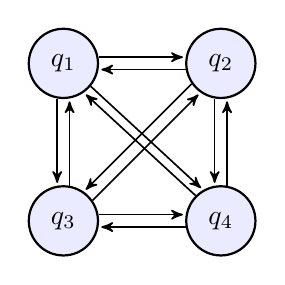
\begin{tikzpicture}[->,>=stealth',shorten >=1pt,auto,node distance=2cm,semithick]
\tikzstyle{every state}=[fill=blue!8,draw=black,thick,text=black,scale=1]

\node[state]         (A)              {$q_{1}$};
\node[state]         (B) [right of=A] {$q_{2}$};
\node[state]         (C) [below of=A] {$q_{3}$};
\node[state]         (D) [below of=B] {$q_{4}$};

\path (A.10) edge  [right] node[right] {} (B.170);
\path (A.260) edge  [right] node[below] {} (C.100);
\path (A.320) edge  [right] node[below] {} (D.120);
\path (B.190) edge  [right] node[left] {} (A.350);
\path (B.215) edge  [right] node[below] {} (C.55);
\path (B.260) edge  [right] node[below] {} (D.100);
\path (C.35) edge  [right] node[above] {} (B.235);
\path (C.80) edge  [right] node[above] {} (A.280);
\path (C.10) edge  [right] node[right] {} (D.170);
\path (D.190) edge  [right] node[left] {} (C.350);
\path (D.135) edge  [right] node[above] {} (A.305);
\path (D.80) edge  [right] node[above] {} (B.280);
\end{tikzpicture}
\end{center}
\caption{Four-state CT Markov model}
\label{fig:msm}
\end{figure}

The intensity matrix for Figure~\ref{fig:msm}, $Q$, represents the instantaneous behavior of the process $X$, and the associated set of model intensities.
\begin{figure}[h!]
\begin{center}
\[
Q_X =
  \begin{bmatrix}
    q_{1,1} & q_{1,2} & q_{1,3} & q_{1,4}\\
    q_{2,1} & q_{2,2} & q_{2,3} & q_{2,4}\\
    q_{3,1} & q_{3,2} & q_{3,3} & q_{3,4}\\
    q_{4,1} & q_{4,2} & q_{4,3} & q_{4,4}\\
  \end{bmatrix}
\]
\end{center}
\caption{Intensity Matrix}
\label{fig:q}
\end{figure}


To illustrate this idea, I begin with a discrete time example.  Suppose a 

\subsubsection{Representation}
The specific instance of CT-Markov models we use for temporal abstraction are based on multi-state Markov models (MSMs).  Similar to a dynamic Bayesian network, arrows represent the allowable transition between model states, which are quantified by an \emph{instantaneous risk}, or transition intensities.

MSMs can be viewed as a domain specific instance of the larger class, where the semantics of the model structure has an interpretation that is rooted in epidemiology and biostatistics.  The models share the same mathematical foundations rooted in homogenous time stochastic processes, but have evolved separately from the theoretical and applied work in computer science on CT-BNs.

This class of CT-Markov models have been applied for the modeling of numerous chronic diseases including HIV~\cite{Presanis11}, lung disease~\cite{Titman10}, hepatitis~\cite{Sweeting10}, and others for over ten years.  One model is learned from the set of all patient observations and used to describe a population-level disease phenomena.  In addition to the base Markov model, they have hidden and semi-Markovian extensions ~\cite{Jackson2011} and there is various work that aims to improve on model optimization techniques.




\subsubsection{Learning}
The probabilities of transitioning are a function of time and transition intensity.  When the values are unknown, maximum likelihood estimates for the parameters, priors for the model, can be computed from the probability matrix, $P(t)$ that is evaluated in a time interval $(0,t)$ is based on the Kolmogorov differential equations and explained by the relationship $P(t)= exp(tQ)$ (cite Taylor and Karlin, 1994).  When there are relatively few states, an analytic solution can be found.  


\subsubsection{Inference}



\subsection{Multi-state Markov Models}

\section{Pairing Nonparametric Clustering}
A variety of researchers have pointed to the limitations of casting clustering as a partitioning problem, where number or clusters are known $a priori$.  Not only does this suggest that the categories exist independently of problem context, and the size and complexity of the data set, but it can force the membership of observations into meaningless clusters, and lead to spurious clusters.

For example, methods that determine the number of clusters $k$ are heuristics and often produce unsatisfying results.  However, research shows that humans employ multiple strategies for finding $k$, and even on simple data sets the number of possible interpretations can be high~\cite{Lewis09}.

\subsection{Spectral Clustering}
Many varieties of spectral clustering algorithms exist and in this work we use a method first proposed by Ng et al.~\cite{Ng01onspectral}, which builds upon existing work by normalizing the Laplacian affinity matrix before eigenvalue decomposition and selection of $k$ largest eigenvalues.

More background on spectral clustering can be found in Chapter X.  A an outline of this approach is as follows:

\begin{itemize}
\item Create the affinity matrix $A$ defined by $A_{ij} = exp(-||s_i-s_j||^2/2 \sigma^2$ if $i \neq j$ and $A_{ii}=0$
\item From $A$ define $D$ as the diagonal matrix where $D_{ii}$ is the sum of the $i$th row
\item Construct the matrix $L=D^{-1/2}AD^{-1/2}$
\item Find the $k$ largest eigenvectors of $L$, $\{s_1,...,s_k\}$ and form the matrix $S$ by stacking them
\item Define the matrix Y by renormalizing each row in $X$ and perform $k$-Means (or another clustering method) to obtain a clustering assignment $C=\{c_1,...,c_k\}$
\item For each initial point $x_i$ where $i \in \{1,...,n\}$, if row $i$ of the matrix $Y$ was assigned to the cluster $j$ where $j \in \{1,...,k\}$
\end{itemize}


\subsection{Nonparametric Bayesian Clustering}
Bayesian approaches for modeling require that a prior on the distribution is assumed.  One way to model uncertainly in this prior is to use a nonparametric approach, meaning one that allows the parameters used to describe the prior adapt to the complexity of the data.  One flexible prior for modeling mixtures is the Dirichlet prior.

These methods typically work by assuming that the process is generated by a potentially infinite amount of parameters, but that for any finite sample can be expressed by a finite number of parameters that are exhibited as a function of a sample-specific characteristic.  In the case of clustering this is the number of components in a mixture model, $k$.

There are certain properties of data sets that make these assumptions more true and problems where the flexibility is desirable in modeling.  For example, in many real-world data sets the number of clusters is dependent on the sample size.  Demographic research shows that as population size grows so does the variability of demographic categories and it unnatural to fix $k$, a priori.  Also, determining $k$ is a challenge posed by many traditional clustering algorithms.

In addition to abstraction with a continuous-time model that draws from work from Bayesian networks, stochastic processes and disease progressing modeling, we extend the clustering component to the \emph{nonparametric Bayesian setting}.  This allow for the number of clusters to be expressed as a function of the sample size, and lending a more natural interpretation to a domain expert.  Specifically, we apply Dirichlet Process Gaussian Mixture Models for determine the number of states in a CT-model and to cluster temporal abstractions.

To compute the model likelihoods and posterior distribution of the clusters we used a mean variational inference for the infinite Gaussian mixture model instead of Gibbs sampling using (Pedregosa 2011).


%Data Sampling and Incompleteness in Health Records}
%section{Modeling Chronic Disease Trajectories} z
%To provide a better understanding of dynamic changes that can occur during the course of a patient�s disease trajectory, this work applies exploratory analysis methods to temporal data. One major challenge posed by modeling patient level data is that disease related observations are typically documented only during hospital or physician visits, resulting in irregular time intervals. Also, a patient�s measurement sequence be short or can span over many years and the nature of the observation scheme (e.g., fixed, random or selfselected) can be unclear.


\subsection{Adaptation to New Problem Tasks}
Lastly, to keep pace with the proliferation of data, learning methods that can separate problem semantics and algorithmic components facilitate reuse.  We not only describe a new temporal clustering method to more accurately represent continuous-time data that does not fit the canonical form of a time series, but similar to other problems based on the expressive language of DBNs, flexible enough to adapt to new problem semantics with little algorithmic tuning.



\chapter{Experiments}
\label{ch:expts}
\chapter{Application: Chronic Hepatitis}
\label{ch:expts}


%Using lab test values reported for a population of patients with hepatitis B and C, my first experiment aims to group hepatitis patients with similar stages of liver decline by modeling the dynamics of the lab test indicates associated with liver disease progression.  The second data set is not composed of actual lab values, rather a higher-level signal that can be captured in administrative records.  For a population of patients admitted to New York Presbyterian hospital, this data physicians orders for glucose tests during hospital stays and aims to group patients that are at high and low risk of diabetes associated hospitalizations.


\section{Application: Grading and Staging Liver Disease}
\subsection{Background}
`Hepatitis' is a Greek word with the root `hepat' meaning liver and the suffix `itis' indicating inflammation.  It is used to describe a class of viruses that are associated with liver inflammation and is characterized by three main types, A, B and C.  Hepatitis A is associated with acute inflammation of hepatocytes (`cyte' is a suffix meaning cell), and types B and C, chronic inflammation.  Individuals with types B and C have the potential risk of developing more severe stages of the disease that may result in permanent scaring of liver tissue, a condition known as cirrhosis, and hepatocarcinoma, a common type of liver cancer.

An indicter of cirrhosis or hepatocarcinoma is fibrosis of the hepatocytes.  A liver biopsy is the gold standard for the prognosis and treatment of hepatitis B and C and provides information that is used monitor disease progression and inform the treatment of hepatitis B and C patients.     Its primary purpose is to determine the health of the liver by measuring the degree of inflammation and stage of fibrosis.  Two common assessment tools are the Metavir test are shown in Table~\ref{metavir} and the Histologic Activity Index (HAI) shown in Table~\ref{hai}.  The Matavir score gives an indication of the amount of scarring, or fibrosis.  HAI represents an activity level, that corresponds with hepatocyte inflammation.

\begin{table}[ht]
\caption{Metavir Fibrosis Scoring}
\label{metavir}
\vskip 0.15in
\begin{center}
\begin{tabular}{p{0.05\linewidth} p{0.6\linewidth}}
\hline
\textbf{Score}	&  \textbf{Assessment} \\
\hline
0         & no scarring\\
1         & minimal scarring\\
2	     & scarring has occurred and extends outside
 the areas in the liver that contains blood vessels\\
3	     & bridging fibrosis is spreading and
 connecting to other areas that contain fibrosis \\
4	     & cirrhosis or advanced scarring of the liver\\
\hline
\end{tabular}
\end{center}
\vskip -0.1in
\end{table}

\begin{table}[ht]
\caption{Histologic Activity Index}
\label{hai}
\vskip 0.15in
\begin{center}
\begin{tabular}{ll}
\hline
\textbf{Score}	&  \textbf{Assessment}\\
\hline
0 & no inflammation  \\
1-4 & minimal inflammation  \\
5-8 & mild inflammation  \\
9-12 & moderate inflammation  \\
13-18 & marked inflammation  \\
\hline
\end{tabular}
\end{center}
\vskip -0.1in
\end{table}

Although it provides important clinical information to guide the care of chronic disease patients, biopsy is invasive, costly and subject to complications.  Biopsy involves extracting a tissue sample of at least $2-3$ cm in length with a 16-gauge needle that is inserted between two of the patients ribs.  The procedure has been association with complications that can be potentially life-threatening.  Also, can cost hundreds of dollars, and is subject to diagnostic error~\cite{Castera2012}.   For these reasons, alternatives for assessing the stage of liver fibrosis are in great demand and the lack of alternative assessment methods has been noted as a major limitation in both management and research in liver diseases.

\subsubsection{Temporal Indicators}
The progression from chronic hepatitis to hepatocarcinoma via liver cirrhosis is mainly observed in hepatitis C patients.  However, the detailed mechanism of this disease trajectory is not well-understood.  Recent work (cite) has demonstrated that temporal patterns associated with hepatitis indicators can provide useful information about liver activity for predicting fibrosis and present a viable option to more invasive testing.  These indicators are recorded as part of a standard liver panel, a collection of tests that are preformed together and provide useful information to assess liver damage, or urinary tests.

\input{7_1_1_method_data}

\subsection{Abstraction}
\subsubsection{CTBN Model Structure}
A CTBN was used to abstract temporal information and is shown in Figure~\ref{msmgraph}.  The lab results for each patient over time were mapped to corresponding \emph{low}(L), \emph{normal}(N) and \emph{high}(H) values based on thresholds identified by clinical experts, and used as states in the model.  Table~\ref{hepxtab} shows the probability of each transition type based on the frequencies all patient transitions for platelet test values.  For example, based on reported transitions, patients reporting a high platelet count show the following probabilities for their next next observation period: high 92\%, normal 83\% and low is less than 1\%.
\emph{can we provide that averages for all patients here?}

\begin{figure}
\begin{center}
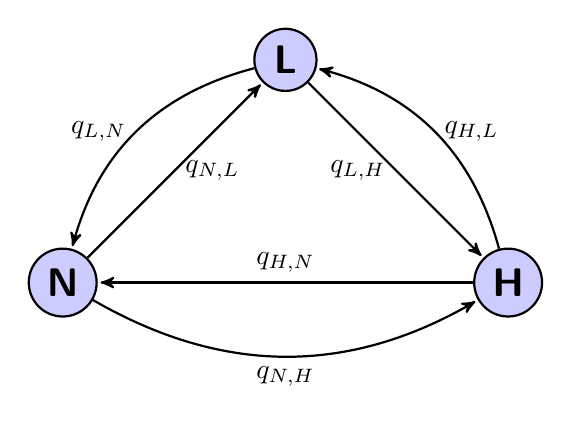
\begin{tikzpicture}[->,>=stealth',shorten >=1pt,auto,node distance=4cm,
  thick,main node/.style={circle,fill=blue!20,draw,font=\sffamily\Large\bfseries}]

  \node[main node] (1) {L};
  \node[main node] (2) [below left of=1] {N};
  \node[main node] (4) [below right of=1] {H};

  \path
    (1) edge node [left] {$q_{L,H}$} (4)
        edge [bend right] node[left] {$q_{L,N}$} (2)
    (2) edge node [right] {$q_{N,L}$} (1)
    	edge [bend right] node[below] {$q_{N,H}$} (4)
    (4) edge node [above] {$q_{H,N}$} (2)
        edge [bend right] node[right] {$q_{H,L}$} (1);
\end{tikzpicture}
\end{center}
\caption{3-state MSM}
\label{msmgraph}
\end{figure}

\begin{table}[ht]
\caption{Input for model abstraction step}
\label{hepxtab}
\vskip 0.15in
\begin{center}
\begin{tabular}{ l | c | c |c}
 $q_{i,j}$      & H & N & L  \\
\hline
H  & 0.915 & 0.083 & 0.001  \\\hline
N  & 0.035 &0.961 &0.004 \\\hline
L   & 0.025 &0.224 &0.751  \\
\end{tabular}
\end{center}
\vskip -0.1in
\end{table}

\subsubsection{Model Variables}
Based on an initial run using six lab tests that were selected due to known associations with liver decline, three, the PLT, ALB, and ZZT tests, resulted in good cluster assignments, with PLT performing the best based on the b-cubed metric~\cite{Bagga}, which is discussed in more detail in Section X, and is the harmonic mean of the average pointwise precision and recall for the cluster assignments compared with a gold standard.

To compare our results with previously published results I cluster patients based on PLT data alone, and in the multivariate lab test data.  To select additional indicators that are most useful, we generated preliminary clustering results using the five indicators that had been reported to have predictive qualities by unsupervised or supervised learning methods.  Using the variables that produced comparable results with that of PLT only, we calculated the mutual information between clusters assignments, and excluded ChE and D-BIL on this basis.  For multivariate temporal clustering of temporal ALB and PLT  data imporved results were achieved compared with results based on PLT alone, and ZZT made a minor improvement upon the results of ALB-PLT based clustering.

\subsubsection{Learning}
Multiple variables are combined for clustering, but the temporal data for each is abstracted separately.  Although the language of CTBNs allows for covariances, they must appear be observed concurrently, and there are numerous time days where the data does not appear for all three.  For example, a patient may have been given both a blood and urine test during a visit, or only one of these at a particular time.

%in the results discuss the strength and limaitaions of this apprach

The continuous time extension to the Baum Welsh algorithm, used the Kolmorgorox equations, which map the transition matrix of a discrete time model to CTBNs. Initial values for the each patients intensity matrix were obtained by using a naive estimation provided by counting the total number of transition pairs for the entire population, and estimating their probability of occurrence. Although not all patients were able to have model parameters output by the abstraction method, initial population level estimates allowed more observations to converge using the parameter estimation methods than the same naive initialization assumption at the patient level.

Using a 4-state multi-state Markov model, each patient's parameters are calculated using likelihood estimations based on the time and values in their observation sequences.  The parameter, or abstraction, used as input to clustering is the matrix $Q$, representing the instantaneous behavior of the process $X$, as an $n$x$n$ matrix.
The model is initialized using To learn the priors for each patients model, using BFGS.




\begin{table}[ht]
\caption{Input for model abstraction step}
\label{hepinput}
\vskip 0.3in
\begin{center}
\begin{tabular}{lcc}
\hline
data& state	& PLT	\\
\hline
19811111& 2&177 \\
19830720&2&182 \\
19830818&2&167 \\
\hline
\end{tabular}
\end{center}
\vskip -0.1in
\end{table}



\subsubsection{Inference}
\subsubsection{Model Comparison}
\subsection{Clustering}


\subsection{Validation}
\label{hep_results}
To validate the results of clustering temporal lab data for the hepatitis data set, we used grading and staging data from liver biopsies a gold standard.  We validate our results using the b-cubed metric and compare performance with results that of previous work using temporal PLT data alone~\cite{Hirano05}, and multivariate temporal data, including PLT-ALB data~\cite{ Hirano07a,Hirano07b} and work publishes in 2012, which extended the approach to PLT, ALB and ChE tests~\cite{Tsumoto12}.  These prior studies used a feature-based technique, ``\emph{trajectory mining}", and provide results that show that compared with conventional studies the method provides a more detailed classification of temporal trends.

I also compare results for alternative clustering algorithms for the semiparametric framework.  Typically, spectral methods are the nonparametric clustering technique of choice.  However, they have some limitations that are discussed in more detail in Chapter~\ref{5_cluster_alg}.  As an alternative, I compare results obtained with spectral clustering with that of Drichlet process Gaussian mixture models, an approach that has its foundation in density estimation and has more recently applied for clustering.  The motivation for applying nonparametric Bayesian for clinical data is described in Chapter\ref{6_extending}.

Lastly, to provide some context for the choice of previous work to focus on only those patients with HVC and no interferon therapy, one needs to be aware of affect on relevant biomarkers.  HVC was considered an nontreatable disease until interferon therapy.  Although beneficial for some patients, there can be serious side effects.  In terms of diabetes indicators, it can cause fluctuations.  Therefore, is can be helpful to distinguish the population of patients with no interferon treatment.

\subsubsection{Comparison of Bayesian and Spectral Methods}
First, we compare alternative nonparametric methods for the semiparametric clustering of temporal hepatitis data, specifically spectral clustering and Bayesian clustering.  Figure~\ref{allHep} visualizes the validation scores reported in Table~\ref{allHepTable}.

\begin{figure}[ht]
\vskip 0.2in
\begin{center}
\centerline{\includegraphics[width=\columnwidth]{fig/allHep.jpeg}}
\caption{B-cubed value for different nonparametric clustering methods and $k$ values for the hepatitis data set}
\label{allHep}
\end{center}
\vskip -0.2in
\end{figure}


\begin{table}[ht]
\caption{B-cubed value for spectral (SP-SC) and nonparametric Bayes (SP-B) clustering, all hepatitis patients.}
\label{allHepTable}
\vskip 0.15in
\begin{center}
\begin{small}
\begin{sc}
\begin{tabular}{lcccr}
\hline
\hline
method	& k	& P	& R	& B-Cubed \\
\hline
\hline
spectral methods & 6	& 0.38& 0.22& 0.28\\
spectral methods	         & 7	& 0.38& 0.21& 0.27\\
\textbf{Bayesian clustering}       & \textbf{4}	& \textbf{0.35}& \textbf{0.62}& \textbf{0.45}\\
Bayesian clustering	     & 5	& 0.35& 0.52& 0.42\\
Bayesian clustering	     & 6	& 0.36& 0.46& 0.40\\
\hline

SP-B	     & 7	& 0.36& 0.42& 0.39\\
\hline
\end{tabular}
\end{sc}
\end{small}
\end{center}
\vskip -0.1in
\end{table}



\subsubsection{Platelet Data}
Using \emph{only} platelet tests, Figure~\ref{plt_only} shows the results of semiparametric Bayesian clustering reported in Table~\ref{pltdatatable}.  The results are compared to techniques developed by Hirano et al.\cite{Hirano05}, and based on b-cubed values that were calculated using the cluster constitutions that were published in their paper, with the authors indicating that small clusters of $n \l 3$ omitted.

\begin{figure}[ht!]
\vskip 0.2in
\begin{center}
\centerline{\includegraphics[width=\columnwidth]{fig/plt_only.jpeg}}
\caption{Comparison of clustering methods using temporal PLT data}
\label{plt_only}
\end{center}
\vskip -0.2in
\end{figure}

%Bayesian clustering	hepC_noInf	plt	5	0.491029213	0.411852866	0.447969438
%Hirano 2007b	hepB	plt	8	0.256698688	0.277312663	0.308345178
%Hirano 2007b	hepC_noInf	plt	6	0.455202852	0.385447555	0.417431134
%Hirano 2007b	hepC_Inf	plt	11	0.386774601	0.229170177	0.28780893
%BC all 	    5	0.330556375	0.386385095	0.356297025	472	
%BC hepC_noInf	5	0.491029213	0.411852866	0.447969438	94	
%BC all         8	0.370831073	0.348019617	0.359063405	472	
%BC hepC_noInf  6	0.477650748	0.424699113	0.449621278	94	
%BC all 	    4   0.357703975	0.38512469	0.370908229	472	
\begin{table}[ht]
\caption{Precision, recall, and B-cubed scores for alternative systems using only temporal PLT data.}
\label{pltdatatable}
\vskip 0.15in
\begin{center}
\begin{tabular}{lccccr}
\hline
\hline
method	& sample &k	& P	& R	& B-Cubed \\
\hline
\hline
Bayesian clustering	& HVC no Tx & 5& 0.49& 0.41& 0.45 \\
Bayesian clustering	& HVC no Tx & 6& 0.48& 0.42& 0.45 \\
Bayesian clustering	& all & 4& 0.36& 0.39& 0.37 \\
Bayesian clustering	& all & 5& 0.33& 0.39& 0.36 \\
Bayesian clustering	& all & 8& 0.37& 0.35& 0.36 \\
Hirano 2005 & HVC no Tx   & 6& 0.46& 0.39& 0.42 \\
Hirano 2005 & HVC Tx   & 11& 0.39& 0.23& 0.29 \\
Hirano 2005 & HVB   & 8& 0.26& 0.28& 0.31 \\
		
\hline
\hline
\end{tabular}
\end{center}
\end{table}


\subsubsection{Hepatitis C, No Interferon Therapy}
\label{hep_results_noinf}
Figure~\ref{hepC_noinf_fig} shows the results of alternative clustering methods on the HCV population with no indication of interferon therapy.  Detailed scores appear in Table ~\ref{hepC_noInftable}.

\begin{figure}[ht!]
\vskip 0.2in
\begin{center}
\centerline{\includegraphics[width=\columnwidth]{fig/hepC_noInf.jpeg}}
\caption{Comparison of semiparametric clustering with a various benchmarks}
\label{hepC_noinf_fig}
\end{center}
\vskip -0.2in
\end{figure}

\begin{table}[ht!]
\caption{Validation scores for HVC patients, no interferon therapy}
\label{hepC_noInftable}
\vskip 0.15in
\begin{center}
\begin{tabular}{lcccr}
\hline
\hline
method	& k	& P	& R	& b-cubed \\
\hline
\hline
Hirano 2007	& 8& 0.60& 0.31& 0.41 \\
\textbf{Tsumoto 2012}	& \textbf{9}& \textbf{0.57}& \textbf{0.33}& \textbf{0.42} \\
\textbf{Bayesian clustering}	& \textbf{4}& \textbf{0.47}& \textbf{0.55}& \textbf{0.51 }\\
Bayesian clustering	        & 5& 0.50& 0.47& 0.48 \\
\textbf{Bayesian clustering}	        &\textbf{ 6}& \textbf{0.48}& \textbf{0.54}& \textbf{0.51} \\
\hline
\hline
\end{tabular}
\end{center}
\end{table}

 Semiparametric Bayesian clustering improves on trajectory mining methods using temporal PLT and ALB data, which showed a 42\% b-cube value~\ref{Hirano07a,Hirano07b} and work publishes in 2012, which extended the approach to PLT, ALB and ChE data, and reports a cluster composition that corresponds with a 42\% b-cubed value ~\cite{Tsumoto12}.

%UPDATE the table
%Bayesian clustering	hepC_noInf	alb-plt-zzt	4	0.466122023	0.554483985	0.506477906
%Bayesian clustering	hepC_noInf	alb-plt-zzt	5	0.495159527	0.469947497	0.482224198
%Bayesian clustering	hepC_noInf	alb-plt-zzt	6	0.476378599	0.538087179	0.505356065
%Bayesian clustering (PLT)	hepC_noInf	plt	5	0.491029213	0.411852866	0.447969438
%Hirano 2007b (PLT)	hepC_noInf	plt	6	0.455202852	0.385447555	0.417431134
%Tsumoto 2012	hepC_noInf	alb-che-plt	9	0.567928605	0.328279479	0.416062542
%Hirano 2007a	hepC_noInf	plt-alb	8	0.5956	0.3097	0.4075


\subsubsection{Semiparametric Bayesian Clustering}
To more thoroughly assess the performance of semiparametric clustering using gold standard results, Figure~\ref{spBayes} shows results for all patients, and the subset of patients with HVC, using temporal data from temporal PLT, ALB and ZZT data. The precision is on the $x$-axis and the recall on the $y$-axis.  The b-cubed values range from dark to light, with lighter values indicating higher scores.

Table~\ref{spbdatatable} reports the results shown in~\ref{spBayes}.  Notably, the best assignment for HVC patients with no interferon therapy reported an 51\% B-cubed for $k=4$ with results for $k=6$ close behind.  For clustering all patients, the results show a 45\% B-cubed value for $k=4$.

\begin{figure}[ht]
\vskip 0.2in
\begin{center}
\centerline{\includegraphics[width=\columnwidth]{fig/spBayes.jpeg}}
\caption{Comparison of semiparametric Bayesian clustering by patient population}
\label{spBayes}
\end{center}
\vskip -0.2in
\end{figure}

\begin{table}[ht]
\caption{Precision, recall, and B-cubed scores for semiparametric Bayesian clustering.}
\label{spbdatatable}
\vskip 0.15in
\begin{center}
\begin{tabular}{lcccr}
\hline
\hline
method	& k	& P	& R	& B-Cubed \\
\hline
\hline
All Pts	& 4& 0.35& 0.62& 0.45 \\
All Pts & 5& 0.35& 0.52& 0.42 \\
All Pts & 6& 0.36& 0.46& 0.40 \\
All Pts & 7& 0.36& 0.42& 0.39 \\
		
\hline
\hline
HVC no Tx	& 4& 0.47& 0.55& 0.51 \\
HVC no Tx & 5& 0.50& 0.47& 0.48 \\
HVC no Tx & 6& 0.48& 0.54& 0.51 \\

\hline
\end{tabular}
\end{center}
\end{table}

%Bayesian clustering	all	alb-plt-zzt	4	0.351527266	0.622462748	0.449311851
%Bayesian clustering	all	alb-plt-zzt	5	0.352476136	0.518519429	0.419670851
%Bayesian clustering	all	alb-plt-zzt	6	0.356380466	0.458481777	0.401034532
%Bayesian clustering	all	alb-plt-zzt	7	0.358414504	0.420788916	0.387105207
%Bayesian clustering	hepC_noInf	alb-plt-zzt	4	0.466122023	0.554483985	0.506477906
%Bayesian clustering	hepC_noInf	alb-plt-zzt	5	0.495159527	0.469947497	0.482224198
%Bayesian clustering	hepC_noInf	alb-plt-zzt	6	0.476378599	0.538087179	0.505356065





%\subsubsection{Discrete versus Continuous Time Abstraction}
%To validate the results of clustering platelet count values for the hepatitis data set, we used grading and staging data from liver biopsies. Figure~\ref{biopsy} show the result from the clustering with the highest highest purity (0.61\%) and obtained using continuous-time HMM abstraction paired with non-parametric Bayesian clustering.  Cluster purity obtained using spectral clustering, was notably lower, reporting a high of $0.40$.  Cluster membership is visualized in relation to highest biopsy grading, and reported by percent of the total for each grade ($n=468$).  A grading of four indicates cirrhosis of the liver or advance scarring. In addition to grading, biopsy activity is commonly used to stage liver disease and visualized in Figure 2. using the fill variation for each pie.

%\begin{figure}[h]
%\centering
%\includegraphics[width=85mm]{fig/hep_2.jpg}
%\caption{Hepatitis Clusters by Biopsy Staging and Activity}
%\label{biopsy}
%\end{figure}

%External data for validating our glucose data set clustering was not available and intrinsic measures based on cluster silhouettes were used to assess cluster quality.  The results of CT-HMM abstraction paired with non-parametric Batesian clustering paired is reported in terms of average silhouette is shown in~\ref{table:sil}.  Spectral clustering was also paired with CT-HMMs.  Although the average silhouette value was overall lower (0.10), one large cluster had a average silhouette higher that that on the max for non-parametric Bayesian clustering.

%\begin{table}[h]
%\caption{Cluster Silhouettes}
%\centering
%\begin{tabular}{|l|c|c|}
%  \hline
  % after \\: \hline or \cline{col1-col2} \cline{col3-col4} ...
%   Cluster& Members & Average Silhouette  \\
%   \hline
%  $C_1$ & 153 & -0.04956 \\
%  $C_2$ & 269 & 0.9416  \\
%  $C_3$ & 132 & 0.1151  \\
%  $C_4$ & 114 & -0.3712 \\
%  $C_5$ & 337 & -0.5460 \\
%  \hline
%\end{tabular}
%\label{table:sil} % is used to refer this table in the text
%\end{table}

%Compared with discrete-time HMM abstraction for the same data set, in previous work (Tamang 2011) we reported over 80 percent of patients with a good (0.60 or above) silhouettes value.  In comparison, continuous-time HMM abstraction report just over half of patients with a good silhouette value (54 percent).
%\subsubsection{Non-parametric Clustering Alternatives}



\subsection{Discussion}
In addition to evaluation of semiparametric Bayesian clustering with a gold standard, the experiments with the hepatitis data set are designed to compare the approach with an alternative spectral clustering step and previous temporal clustering results reported in the literature.  Here, I discuss the key findings based on external metrics and their clinical significance.  Also, I show a visualization technique to aid the interpretation of clustering results that is based on average model parameters for each discovered cluster, or patient group.

\subsubsection{Spectral Clustering Versus Nonparametric Bayesian Clustering}

 By comparing alternative clustering steps for the semiparametric framework, these results indicate a benefit to \emph{Drichlet process Gaussian mixture modeling}, an nonparametric Bayesian clustering, instead of spectral method.  Due to popularity of spectral methods, and reputation for high performance, my expectation was comparable performance.  I suspected the key benefit would be a relaxation of the requirement to indicate $k$ $a$ $priori$ and not a notable improvement in overall performance.

 One explanation for the improved performance is the distribution of the class labels, which is Gaussian.  Spectral methods methods attempt to balance the size of the clusters while minimizing the interaction between dissimilar points, and can bias results towards clusters of equal size~\ref{WhiteS05}.  Many diseases, and disease-related states show Gaussian population distributions, and our results suggest that spectral clustering may not be the best choice for modeling patient populations.

\subsubsection{Comparison with State-of-the-Art Methods}
To compare the results of semiparametric Bayesian clustering with previous work, I reconstructed a univariate and multivariate experiments and compared them with published results~\cite{Hirano05,Hirano07a,Hirano07b,Tsumoto12}.  I show that it out performs alternative methods for range of scenarios, including univariate and multivariate analysis, and different hepatitis disease types.

Using the best temporal indicator, PLT, results for univariate temporal clustering were small (42\%~\cite{Hirano05} to 45\%).  However it is important to note that in comparison experiment, small clusters where $N$<$3$ were not provided in the membership table.  How generous the score calculated from their cluster constitution table is unclear.

For multivariate temporal data, clustering performance increases over a 20\% relative improvement using combined ALB-PLT-ZTT tab results, reporting a 51\% b-cube score.  Cluster constitutions reported in the literature based on trajectory mining, reported scores between 41-42\% and were based on the temporal modeling of features from combined ALB-PLT~\cite{Hirano07a,Hirano07b} and ALP-PLT-ChE lab data~\cite{Tsumoto12}.

Again, some of the comparison estimates are generous.  The clusters where $N$ < $2$ for the temporal ALP-PLT data results were not provided in the membership table, or could be determined by another reported statistic.  Inclusion of even one of the missing clusters would have reduced the completeness constraint, and lowered the value of the validation metric.

\subsubsection{Clinical Context and Relevance}
The goal of temporal mining task was to discover patient groups that are useful or meaningful to:
 \begin{itemize}
   \item discriminate between those that progress to more advances stages such as cirrhosis or hepatocarcinoma, and
   \item determine if less invasive diagnostic procedures can replace liver biopsy.
 \end{itemize}

In addition to cluster membership, semiparametric Bayesian clustering provides us with additional information for learning group level properties from members' trajectories.  The subpopulation characteristics can be used to assign a unseen patient to one of the discovered clusters.   More specifically, each patient's model parameters characterizes their rate of change from of the disease states to all others.  In Figure\cite{fig:hepq} we show averages for each cluster's characteristic model, based on a three state (low,normal,high) $k=4$ PLT based clustering results.

%1       1  0   4.649329  -9.866057 -41.078529  0 -18.21271 -9.058329 11.266929
%2       2  0  -4.832645 -19.860027  -6.281500  0 -16.76764 -8.736268 -1.768516
%3       3  0 -34.752063 -23.149088   5.142881  0 -14.15912  1.595881 -5.364187
%4       4  0  15.124626   8.949241 -59.671174  0 -27.21240 -8.355130 17.715889


\begin{figure}
\[Q_1= \left( \begin{array}{ccc}
0 & 4.65 & -9.87 \\
-41.08 & 0 & -18.21 \\
-9.06 & 11.27 & 0
\end{array} \right)
%
Q_2= \left( \begin{array}{ccc}
0 & -4.83 & -19.86 \\
-6.28 & 0 & -16.77 \\
-8.74 & -1.76 & 0
\end{array} \right)
\]
\[ Q_3= \left( \begin{array}{ccc}
0 & -34.75 & -23.15 \\
5.14 & 0 & -14.16 \\
1.60 & -5.36 & 0
\end{array} \right)
%
Q_4= \left( \begin{array}{ccc}
0 & 15.12& 8.95 \\
-59.67 & 0 & -27.21 \\
-8.36 & 17.72 & 0
\end{array} \right)
\]
\caption{Intensity Matrices for 3-state, 4 cluster hepatitis model}
\label{fig:hepq}
\end{figure}

The cluster composition is shown by fibrosis stage, the gold standard class used for external validation, appears in Table\ref{hepassignments}.  Fibrosis stages are labeled F0 through F4, with F4 indicating end-stage liver disease.


\begin{table}[ht]
\caption{Cluster composition by fibrosis stage}
\label{hepassignments}
\vskip 0.15in
\begin{center}
\begin{tabular}{lcccr}
\hline
\hline
	& $F0,F1$ &$F2$	& $F3$	& $F4$ \\
\hline
\hline
$k_1$ & 5& 2& - & - \\
$k_2$ & 17& 11& 6& 10 \\
$k_3$ & 6& 1& 3& 6\\
$k_4$ & 25& 1& -& 1\\
		
\hline
\hline
\end{tabular}
\end{center}
\end{table}

\subsubsection{Risk of End-stage Liver Disease}
\label{risk}
To \emph{stratify discovered groups by risk types}, I examine the proportion of class labels within each.  Figure~\ref{hep_2} shows the cluster composition as a percent of total records for each class.  The size of each circle is proportional to the total count for each Matavir score, or class label. Also, it shows the biopsy activity, HAI, with the darkest color indicating the highest activity, and which some consider a better indicator for liver fibrosis than the Matavir score.

\begin{figure}[t]
\vskip 0.2in
\begin{center}
\centerline{\includegraphics[width=\columnwidth]{fig/hep_2.jpg}}
\caption{Metavir biopsy grade and Hepatitis Activity Index (HAI) by cluster as a percent of total records for each class}
\label{hep_2}
\end{center}
\vskip -0.2in
\end{figure}

Based on Figure~\ref{hep_2}, we can broadly rank clusters by increased risk for progressing to end-stage liver disease: $c_4 < c_1 < c_2 < c_3$.  In in $c_1$, the presence of the largest circle at the lowest grade, F0, and a steady decrease in size as biopsy grades increase, indicates the highest composition of patients at low risk.  Consistent with this conclusion, relative to other clusters, $c_1$ patients have a lower activity with only a small fraction showing high biopsy activity.  Similar to $c_1$, $c_4$ also shows the presence of patients with lower biopsy grades, and low activity.  However, it does not show the a larger proportion of these patients at lower biopsy grades, as in $c_1$, suggesting that members of $c_4$ progress to end-stage liver disease more often that those patients in $c_1$, but based on cluster composition, less often that patients in $c_2$, or $c_3$.  Patients in $c_2$ are the most likely to progress to higher fibrosis stages, showing the highest proportion of patients with F3 and F4 scores, that decrease as the fibrosis grade gets lower.  A similar trend is observed in $c_3$ but is not as dramatic.

\begin{figure}[ht!]
\vskip 0.2in
\begin{center}
\centerline{\includegraphics[width=\columnwidth]{fig/hepc_qmatrix.jpeg}}
\caption{Comparison of semiparametric clustering with a reported benchmark}
\label{hepCqmatrix}
\end{center}
\vskip -0.2in
\end{figure}

\subsubsection{Hepatitis Disease Trajectory}
  The irregular sampling of disease related indicators, and the long progression times are obstacles to providing more detailed mechanism for chnonic diseases trajectory that are not well understood, such as hepatitis.  One benefit of model-based temporal abstraction with Bayesian network is that unlike feature-based methods that aim to characterize salient properties of the observed signal, they provide a direct representation of the underling process or phenomena they model.

  For non-canonical time series data, continuous-time Bayesian networks (CTBNs) can provide parameters for patient and population level models that can be used to provide insight into chronic disease progression, specifically, the instantaneous rate of change between of this disease states.  The added benefit of clustering is the division of a patient sample into subpopulations that can correspond with meaningful groups such as risk types, providing the ability to examine hepatitis trajectories at a finer-level of detail that is useful for characterizing patients.

  Figure\cite{fig:hepq} shows a characteristic intensity matrix for each of the clusters. To facilitate their interpretation, and compare clusters in terms of instantaneous risk factors, Figure~\ref{hepCqmatrix} visualizes the each of the intensity matrices.  Each cluster is represented by a color along the $y$-axis, and the $x$-axis represents the the number of standard deviations each cluster's dataum is relative the mean for all of the $q_{ij}$.  Each of the nine plots in the 3x3 grid that correspond with the entries of the $Q$ matrix, and represent the transitions from low, normal and high disease states.

Based on our assessment of risk types in Section~\ref{risk} that broadly qualified the clusters by increased risk of end-stage liver disease as $c_4 < c_1 < c_2 < c_3$, we can describe properties of patient sub-populations in terms of instantaneous risk, and relative to each other.  For example, if a patient is currently in a normal state, how likely are they to progress to lower (unhealthy) state?  Figure\cite{fig:hepq} shows us the model parameters for each cluster, and indicated the precise value of the instantaneous risk.

To compare sub-populations relative to each other, the $q_norm,low$ entry in Figure~\ref{hepCqmatrix} shows us that patients in $c_1$ and $c_4$, which correspond with those at less risk of fibrosis, are more likely to remain in the normal state, and patients in  $c_1$ and $c_4$, the patient groups with the highest fibrosis risk, are more likely to transition to poorer health based on the population average. Also, it shows that $c_4$ represents patients are mostly likely to remain in a normal state and $c_3$ patients are the most likely to transition to a poorer health states.  Notably, this interpretation is consistent with our designation for risk types, and their rank from lowest to highest risk, and can be made for other key model transitions.

\subsubsection{Actionable Findings}
One important finding that is not adequately captured by standard evaluation metrics that is relevant to our problem is related to the increased importance of lowest fibrosis class, composed of patients labeled F0 or F1 in the gold standard.  Specifically, liver biopsy is an invasive procedure that can put patients at risk of procedural complications, and costs hundreds of dollars.  The ability to reduce the number of unnecessary biopsies is currently an active area of research.

The lowest risk cluster generated by our procedure consistently produced one cluster of high purity for F0 and F1 patients.  Although this cluster was not maximal for this population, it can be used to identify patients for which biopsy is likely unnecessary.  For example, 93\% of patients in $k_4$  (see Table\ref{hepassignments}) had unnecessary biopsies, and represent about a quarter of the patient sample.





%cluster assignments appear in the NYU slides 


\chapter{Application: Diabetes Monitoring}
\label{ch:expts}
\section{Application: Blood Glucose Maintenance}
National estimates report a 8.3\% prevalence of diabetes in the Unites States, with over seven million undiagnosed~\cite{cdc}.  The disease can result in various health complications such as kidney failure and blindness.  However, medical research shows that behavioral changes and other interventions can prevent or delay diabetes onset showing how importance of early diagnosis and treatment.   \emph{Data mining and  machine learning methods applied to clinical data} have been the focus of a national challenge task, and various research research practice partnerships to predict diabetes risk, and diagnose diabetes over the last decade\cite{Kaggle, HHP}.

The glucose data set is derived from administrative data encounter data that was generated during hospital admissions, and consists of physician ordered glucoses tests.  The clustering application seeks to identify high-level patterns in physicians orders for glucose tests that corresponds with patient sub-populations that they can be examined in more detail.  Although glucose test values would provide a finer-grained detail, the values are sensitive to the time of day that the test was administered, and both they type and time of food or drink ingested before testing.  Also, a higher-level utilization data is more common and accessible to insurance providers and can be generated from a patients claims profile.  Since untreated diabetes can result in more serious conditions, it is in the interest of insurance providers to shift resources towards preventative care.

The glucose test data is for a population of patients admitted to NYPH Hospital with more than one physician ordered glucose test indicated in their EHR. Similar to the hepatitis patient data, the glucose time series presents methodological challenges in that it is irregularly sampled, and variable in length.  Additional complicating factors is an increased probability of record incompleteness and a self-selection sampling mechanism.

In the 2010 the CDC reported that 11.5\% of hospitalizations in the US indicated diabetes as the primary diagnosis\footnote{http://www.cdc.gov/diabetes/statistics/hosp/adulttable1.htm}.  Due to the prevalence of diabetes, and its association with hospital admission, glucose tests are commonly ordered by physicians for hospitalized patients.  It is important to note that physicians' orders for a glucose test does not indicate diabetes, or prediabetes.  They are part of the metabolic panel that may be ordered to assess kidney and other organ health, or the patient may fit an at risk profile.  Therefore, glucose test with out any follow up on the succeeding day may corresponds with a short admission, or with a longer stay that does not require ongoing glucose monitoring. For this reason, it is not the indication of a single, sparse glucose testing that is informative, but rather a series of contiguous testing patterns over time.  For a hospitalized patient, this can suggests that their blood-glucose levels are being actively monitored by the attending physician, and either the patient is diabetic or prediabetic.

\subsection{Data Description}
For each patient, the sequence begins with the first physician ordered by test on record and indicates the presence `1' of a physician's order at $t_1$.  Each successive day, $t_2,t_3,...,t_T$, for a total $T$ days, a daily value indicating the presence or absence `0'  composes the patent's temporal measurement sequence.  At time $T$ measurement sequence is terminated by a censoring state (e.g. death) or on the day the record was extracted from the hospital information system.

Figure~\ref{desc_glucose} shows descriptive statistics for the entire patient population in the glucose data set and including, record length, the entropy of the measurement sequence, total visits, the absence entropy, the fraction of visits, and the length of the longest gap in each patient's measurement sequence.

\begin{figure}[ht]
  \centering
  % Requires \usepackage{graphicx}
  \includegraphics[width=\columnwidth]{fig/histograms_descriptivestats_color_wmeans.jpeg}\\
  \caption{Descriptive Statistics for Patients in the Glucose Data Set}\label{desc_glucose}
\end{figure}

\subsubsection{Selection Criteria}
Although the methods can be applied to larger samples, and other types of samples, in order to compare results visually for assessment, I select patients with a time series length in the range of 1000 to 1025 days, consisting of just over 3 years of daily measurement data.  Figure~\ref{statsXlor} shows the sample in the context of the larger population for several of the aggregate measures that appear in Figure~\ref{desc_glucose}.  The length of record (lor) equal to 1000 is marked by the vertical red dash, and shows that about this lor length the longitudinal measurement patterns begin to exhibit more regular patterns in terms of the entropy of "1" values and of "0" measurement values.  Also, it shows that this population is not an outlier for the number of visits.

\begin{figure}[ht]
  \centering
  % Requires \usepackage{graphicx}
  \includegraphics[width=\columnwidth]{fig/statsXlor.jpeg}\\
  \caption{Comparison of study sample with larger glucose data set}\label{desc_glucose}
\end{figure}

Both of these features suggest this is an appropriate lor to capture longer term chronic disease trends, and avoid some of the computational burden associated with using longer time series for the development of new temporal clustering methods.  Also, unlike alternative nonparametric clustering algorithms, Bayesian clustering does not assume a fixed $k$, and rather a  function of the size and complexity of the data. Therefore the need to extract a sample with enough power to represent all patient groups is less of a concern, and as new samples are drawn this method will estimate $k$ accordingly.

In the collection of patients, our selection criteria resulted in a total of 1024 patient measurement sequences.  The descriptive statistics for the time series sequences for the patient population that meet the selection criteria are shown in Table~\ref{glucoseStats} and the values are visualized in Figure\ref{stats_1000_1025pts}.

\begin{figure}[ht]
  \centering
  % Requires \usepackage{graphicx}
  \includegraphics[width=\columnwidth]{fig/stats_1000_1025pts.jpeg}\\
  \caption{Descriptive Statistics for the Glucose Study Sample}\label{stats_1000_1025pts}
\end{figure}


\subsubsection{Measurement Sequence Transformation}
In contrast to the hepatitis data set, the glucose data set does not reflect raw data values, but a higher level signal with less information.  For discrete time modeling, time slices in the model are represented by the smallest temporal granularity, which in this case is one day.  For example, patient $i$, with $T=15$ and their first glucose test indicated on January 1 and subsequent measurements on the 5th-8th, and again on the 13-15th, would be represented by the measurement sequence $$x_i = [(t_1,1),(t_2,0),(t_3,0),(t_4,0),(t_5,1),(t_6,1),(t_7,1),(t_8,1),
(t_9,0),(t_{10},0),(t_{11},0),(t_{12},0),(t_{13},0),(t_{14},1),(t_{15},1)]$$

Continuous-time models allow for a more direct representation of the temporal phenomena, and do not require a fixed time interval that is the length of the smallest time granularity.    Not only does this allow for a new representation, it more explicitly captures informative features of a measurement sequences including, the contiguous measurements, their density, and frequency.

In contrast to the discrete time model, this approach results in a measurement sequence that is equal to the number of each patients episodes in each patients record.  Since we need only to represent the data that is known, intervening time slices where no tests were observed are not required to be represented.

First, we model each admission as a episode corresponding with a tuple, and instead of the 0/1 indication, the number of contiguous tests is used.  To learn the temporal model for each patient, the values are paired with the start time.  Below is the new representation for $x_i$, $x_i'$,
$$x_i' = [(t_1,1),(t_5,4),(t_14,2)]$$

Also, for discrete time Bayesian networks, when the parameters for a model must be learned, the forward-backward algorithm consists of $T-1$ iterations.   Although the continuous-time version of this algorithm required additional computational steps, when models are sparse, it is much more efficient and this has been noted as a key advantage of continuous-time modeling over discrete time approaches for this type of modeling task.

Figure~\ref{sequence_reps} in the Appendix shows the the representation of the measurement sequence for discrete time modeling and continuous time modeling for two patients in our sample that were separated into two different clusters.  For the first sequence, what would consist of over one thousand iterations of a learning algorithm is reduced to two.  In the second case it is reduced to less than thirty iterations.

\subsection{Abstraction}

\subsubsection{Structure}
For the continuous time, multi-state model, I estimated $n$, the \emph{number of states} for the models using a non-parametric Bayesian density estimator.  A summary of the data that was used as input for state estimation is shown in Figure~\ref{testdurations}. Based on the log likelihoods and resource restrictions a four state model was identified, and provides a mapping for each "observation", or instance of contiguous glucose measurements to one of the four states.

\begin{figure}[ht]
  \centering
  % Requires \usepackage{graphicx}
  \includegraphics[width=\columnwidth]{fig/testdurations.jpeg}\\
  \caption{Distribution of contiguous glucose testing durations Sample}\label{testdurations}
\end{figure}


\subsubsection{Learning}
\subsubsection{Inference}
\subsubsection{Model Comparison}
\subsection{Clustering}


\subsection{Validation}
There is no gold standard for the evaluation of results.  Instead, I assess intrinsic qualities of the generated clusters using both common metrics described in Section\ref{5_clust_alg}, and clinical context about the problem task.

\subsubsection{Semiparametric Bayesian Clustering}
Based on the results of applying our clustering approach to the glucose testing data, Figure~\ref{sil} shows the silhouettes by cluster for a four-state glucose model that generated five clusters.  Of the 1025 initial patients, our parameter learning technique converged, and produced model parameters that were then clusters for 1005 patients.  Each observation's silhouette is grouped by cluster along the y-axis, and members are sorted within each cluster by each assignment's value.

\begin{figure}
\begin{center}
\centerline{\includegraphics[width=\columnwidth]{fig/sil.jpeg}}
\caption{Silhouettes by cluster for 4-state model.}
\label{sil}
\end{center}
\vskip -0.2in
\end{figure}

 The value of 0.6 is generally the threshold for a good cluster in terms of similarity to other members of its own cluster and distinction from members of other clusters.  Table~\ref{glucose_cluster_stats} shows each cluster's size, mean and average silhouette value, and suggests that $c_0$ and $c_1$ are good assignments.

 \begin{table}
\caption{Size, Mean and Median Silhouette Values by Cluster}
\label{gluc_stats}
\vskip 0.15in
\begin{center}
\begin{small}
\begin{sc}
\begin{tabular}{lccccr}
\hline
 	&$c_0$ 	&$c_1$	&$c_2$ 	&$c_3$	&$c_4$ \\
\hline
size	&263	&321	&262	&98	&61\\
mean	&0.8841	&0.7267	&-0.1573	&-0.3669	&-0.3167\\
\hline
\end{tabular}
\end{sc}
\end{small}
\end{center}
\vskip -0.1in
\end{table}

The characteristic $Q$ matrices for each cluster are based on mean of the patient distribution for each model state.  In the four-state model the states reflect increasing disease severity, with the first indicating normal blood-glucose levels. Each $q_{ij}$ corresponds with the instantaneous risk of moving from state $i$ to state $j$.

\begin{figure}
\[Q_0= \left( \begin{array}{cccc}
0     &   -25.55&   -11.09& -14.54\\
14.66 &        0&    -4.74&	  1.55\\
12.72 &     3.84&	     0&  -1.49\\
11.09 & 	3.38&  	-13.87&    0

\end{array} \right)
%
Q_1= \left( \begin{array}{cccc}
0 & -2.28	&-2.83	&-5.3\\
-0.61&  0&	-2.24&	-4.19\\
-0.76&	-1.61&	0 &  -3.72\\
-0.52&	-2.84&	-2.59& 0
\end{array} \right)
\]

\[ Q_2= \left( \begin{array}{cccc}
0& -0.65&	-12.45&	-11.92\\
4.93&    0&	-7.30&	-8.62\\
8.00&	0.37& 0&	-5.60\\
7.15&	-1.31&	-1.52& 0
\end{array} \right)
%
Q_3= \left( \begin{array}{cccc}
0 & -20.04&	-4.64&	-8.17\\
8.98& 0&	-0.36&	-0.46\\
2.95&	-2.13& 0&	-7.31\\
5.52&	0.75&	-2.35& 0
\end{array} \right)
\]

\[ Q_4= \left( \begin{array}{cccc}
0 & -2.76&	-0.39&	-3.85 \\
-13.73& 0&	-5.50&	-7.00 \\
0.35&	0.92&   0&	-2.66 \\
6.38&	-5.97&	2.22& 0


\end{array} \right)
\]
\caption{Intensity Matrices for 4-state, 5 cluster glucose model}
\label{fig:glucq}
\end{figure}

\subsubsection{Cluster Comparison}

To examine patient subpopulation by cluster characteristics, time series statistics for each cluster. is shown in Table~\ref{gluc_stats}.  Reported are the number of total tests (Tests), the number of contiguous blocks of daily tests (Blocks), the entropy of the measurement sequence (Entropy), and the fraction of days measured by cluster (Fraction).

\begin{table}
\caption{Time series statistics aggregated by cluster}
\label{gluc_stats}
\vskip 0.15in
\begin{center}
\begin{small}
\begin{sc}
\begin{tabular}{lccccr}
\hline
k 	&n 	&Tests 	&Blocks 	&Entropy 	&Fraction \\
\hline
0	&263	&8.6	&7.81	&0.05	&0.01\\
1	&321	&39.64	&16.98	&0.14	&0.04\\
2	&262	&22.00	     &13.53	&0.10	&0.02\\
3	&98	    &24.77	&11.38	&0.10	&0.02\\
4	&61	    &16.74	&7.69	&0.08	&0.02\\
\hline
T 	&1005	&24.08	&12.57	&0.10	&0.02\\
\hline
\end{tabular}
\end{sc}
\end{small}
\end{center}
\vskip -0.1in
\end{table}

Two aggregate time series statistics that have been shown to be informative for feature-based clustering, \emph{entropy of the measurement sequence} and the \emph{number of visits} can help to display visual distinctions among the clusters.   Figure~\ref{box_glucose} compares the clusters by these two aggregate measures.


\begin{figure}
\begin{center}
\centerline{\includegraphics[width=\columnwidth]{fig/glucose_k5.jpg}}
\caption{Average entropy and number of visits by cluster}
\label{box_glucose}
\end{center}
\vskip -0.2in
\end{figure}


To further analyze $c_0$ and $c_1$, I visualize the 0/1 measurement vector with a heat map that shows a light color for the presence of a glucose test and black for the absence of a physicians ordered glucose test. Patients of each cluster appear in the order of increasing visits and are represented in full in detail in Figure~\ref{glucose_seq}.

\begin{figure}
\begin{center}
\centerline{\includegraphics[width=\columnwidth]{fig/grid_datavis.jpg}}
\caption{Highest intrinsic quality cluster 0/1 sequences.}
\label{glucose_seq}
\end{center}
\vskip -0.2in
\end{figure}









\subsection{Discussion}
I discuss the key findings based on intrinsic validation of the cluster assignments using silhouette values and clinical context.  In order to interpret the temporal summarization that is provided by the abstraction technique, I visualize distinctions between patient subpopulations based on the clusters that were generated. Their purpose is to aid the interpretation of clustering results that based on average model parameters for the patients assigned to each of the groups.


\subsubsection{Cluster Comparison}

More than half (584) of the entire sample were assigned to the clusters that show high intrinsic validation scores, $c_0$ or $c_1$.  Although the length of all patient records is about three years, observable differences can be seen for for $c_0$ and $c_1$, providing further evidence that these clusters are clinically meaningful.
 
 Figure~\ref{box_glucose} shows differences in terms of the entropy of the measurement sequence by the number of visits.  In my previous work that compared feature-based abstraction methods with model-based methods, these two aggregate statistic were informative for clustering.  The figure shows that patients in $c_0$ have a sequence entropy value that is less than half the average in $c_1$.  Also, they have about four times as less tests overall.  The other clusters fall between these values, with two of them grouping about midway, suggesting that their composition is more heterogenous, or that the have some glucose management issues, but that they do not lead to multiple day hospitalizations where glucose ins continually monitored.
 
 \subsubsection{Diabetes Trajectory}
  This application aims to discover patient groups from the glucose data set that are useful for understanding and defining characteristic groups of patients from temporal diabetes-related data.  
  
   Figure~\ref{glucose_seq}, shows a heat map for  $c_0$  1/0 sequences that is sparse.  The only time multiple daily measurements are observed is at the very beginning of the sequence, and almost no members ever exhibit the most severs state, 4.  The values of the transition matrices (Figure\ref {fig:glucq})also indicate that $c_0$ corresponds with patients that are more likely to maintain blood-glucose values.  In contrast, the $c_1$  1/0 sequences that is more dense, and patients exhibit higher states on average.
  
In order to interpret the abstraction models that provide summarize each patient's temporal characteristics, I visualize the $Q$, or intensity matrix, that is learned for each patient.  In each cluster is represented by a different colored horizontal bar that reflects the z-scaled value for the state and reflects a cluster average.  The 16 plot in Appendix Figure\cite{glucose_qmatrix} correspond with the each of the $q_{ij}$ of the 4x4 intensity matrix.

A temporal trend that is consistent with the better health associated with patients in $c_0$ and poorer health in $c_1$ can be observed.  Figure~\ref{glucose_q1matrix} compares the z-scaled values for the state 1 and it's possible transitions.  It shows that patients in $c_0$, indicated as 1 on the y axis and a salmon color, are more likely to stay in state 1 than transition to higher states, 2,3,or 4 compared with the average.  Patients in $c_1$, indicated as 2 on the y-axis and an olive color,  are the opposite, and more likely to transition the the higher states.  Other clusters, with the exception of $c_4$, which is the smallest cluster and shows a high proportion of patients in higher states, do not show a consistent trend as the states increase.  The characteristic intensity matrices for clusters $c_2$ shows that patients are more likely to stay in $q_1$ than progress to $q_2$ but a small risk of transition to higher states.  The last cluster, $c_2$, indicated by green, and 3 on the y-axis shows the opposite behavior, and an increased risk.

 \begin{figure}[ht]
  \centering
  % Requires \usepackage{graphicx}
  \includegraphics[width=\columnwidth]{fig/q1_glucose.jpeg}\\
  \caption{Characteristic $Q$ Matrices by Cluster}\label{glucose_q1matrix}
\end{figure}
 
 
 Although a clinical significance of $c_2, C_3$ and $c_4$ can be interpreted form the results, it should be considered that these clusters have poor intrinsic quality.  Also, that they are smaller in size, and characteristic $Q$ matrix may be more sensitive to parameter changes as new observations are made available for learning.  Also, these clusters are less distinctive in Figure~\ref{box_glucose}.
\subsubsection{Discrete Versus Continuous Time}


\subsubsection{Clinical Context and Relevance}

 
 



\chapter{Summary}
\label{ch:summary}
\section{Summary}
The experimental methods and study results are presented for two distinct clinical data sets.  The first consists of patient lab data that was collected in Japan at in and outpatient visits, and represents individuals with HVB and HVC.  Our second data set was generated form an inpatient population at a large urban hospital with at least two indications of physician ordered glucose tests during their hospital stay.

The irregular sampling of clinical observations over variable durations is the main challenge for existing temporal mining methods.  The new techniques described in this thesis provide a principled method for their exploratory analysis.  Specifically, they can be used to preprocess patients with the aim of enriching the quality of the data by eliminating observations that are noisy or less relevant for the research purpose, or to discover patient groups that can help detail the natural history of population and subpopulation level disease phenotypes.

Although each study has the goal of reveling inherent patient groups that correspond with disease phenotypes, there are some distinctions between the two sets.  First, the hepatitis data set is more complete, combining both in-patient and out-patient laboratory examinations.  Also, the time of observation is less likely influenced by an informative sampling scheme. In the case of the inpatient glucose monitoring data, it is more likely that sampling time is influenced by self-selection sampling, and driven by the need to seek emergent care.

\section{Modeling Chronic Hepatitis}
 In our experiments, the dynamic patterns that are produced by modeling platelet count over time helps to group hepatitis B and C patients in a way that is useful for informing the prognosis and treatment of patients.  If used as a screening tool, our experiments suggest that for unseen patients that are most similar to our lowest risk cluster, it will likely result in unnecessary biopsies.

 However, for patients at higher risk, our method does not provide sufficient evidence to base prognosis and treatment on the basis of clustering assignments alone.  It does provide useful information for assessing higher risk patients, but associates some lower risk patient, increasing cluster heterogeneity.

 These findings are aligned with recent work in supervised learning~\cite{Jiang2006}, and distinct work in clinical research~\cite{Parkes2011} indicating methods that use noninvasive serological markers to assess fibrosis stage can reduce the number of unnecessary biopsies, or eliminate the need ~\cite{Gangadharan}.  Recent studies use numerous direct and indirect serum markers and even challenge the need for liver biopsy  or replace liver biopsy.  They do not attempt to model dynamic changes that are key to description  a patient trajectory, and instead entail test panels that provide a richer cross-sectional picture.

 For clustering temporal clinical data, the semiparametric Bayesian clustering explicitly models the dynamic changes that occur over the course of a patient's trajectory.  For chronic hepatitis patients, I identify key features for modeling patient disease dynamics by calculating the mutual information between lab tests that have Also, just more variables improve the performance of liver panels for assessing fibrosis, a more articulated abstraction model will also improve temporal clustering performance for identifying various risk strata.




\chapter{Conclusions}
\label{ch:conclusions}
\chapter{Conclusions}
\label{ch:conclusions}

Although there is extensive work on approaches for modeling patients in environments such as the ICU, these do not easily translate to long durations, such as months or years.  To this end, we demonstrate a clustering method for the exploratory analysis of longitudinal patient data that easily extends to new data sets, and in contrast to discrete time approaches, is more appropriate for modeling incomplete, irregular observation sequences that are common to patient data found in electronic health records.

We demonstrate a new method to model patient disease dynamics with two key features.  First, we use continuous-time (CT) HMM abstraction, which avoids some of the limitations of discrete-time approaches when a dynamic process evolves at different time granulations, and when observations are irregularly sampled and missing not at random.  Second, non-parametric Bayesian clustering methods avoid the problem of identifying the number of clusters a priori, inferring the appropriate number of mixture component as a function of the sample size.

Specifically, we apply hidden multi-State models, an instance of continuous-time HMM models used by biostatistican for disease modeling.  Although we were unable to match the intrinsic clustering quality achieved in previous work using discrete-time HMMs abstraction with glucose test data, performance was comparable.  However, on a hepatitis data we externally validate their effectiveness.  We also assess the performance of pairing temporal abstraction with a non-parametric Bayesian clustering.  It conveniently eliminates the need to estimate $k$, and  performed better that spectral clustering on the hepatitis data set.

\section{Future Work}

 Our continued work will focus on more rigorous, and alternative methods for cluster evaluation. Silhouette values are limited in their ability to assess quality and there may be more suitable, or additional methods to evaluate clusters.  Also, in terms of external validation for our hepatitis data set, our clusters are not categorical, but rather ordinal and accounting for the relations between clusters may also provide additional insights into the performance our techniques.

%The accumulation of data has outpaced the development and adoption of tools that can process and analyze data artifacts to present more succinct and informative summaries of interest to end-users.  However, temporal data can provide critical contextual information to discover new knowledge relevant to health and wellness.  However, the accumulation of patient data has outpaced the generation of effective methods for temporal analysis.





\bibliographystyle{plain}
\bibliography{dissertation}

\appendix
\chapter{Appendix}
\begin{table}
\begin{center}
    \caption{Comparison of clustering techniques for sequential data}
\label{hepaticpanel}
\begin{tabular}{| p{2cm} | p{10cm}  |}
  \hline
  \multicolumn{2}{|c|}{\textbf{Laboratory Tests} } \\
  \hline
  \multicolumn{2}{|c|}{Hepatic Function Panel}\\ \hline
  Platelets (PLT) & Platelet counts for hepatitis patients with cirrhosis are low, but can be the result of other causes.  This lab test measures the platelet number in the blood. \\ \hline
  Bilirubin (D-BIL) & This test measures the bilirubin level in the blood, and is produced by the breakdown of hemoglobin. If the liver is not functioning correctly, it will not be properly excreted.\\ \hline
  Colinesterase (CHE) & Michael Duberry \\ \hline
  \multicolumn{2}{|c|}{Urine Test}\\ \hline
  DC & Dominic Matteo \\ \hline
  RB & Dider Domi \\
  \hline
\end{tabular}
\end{center}
\end{table}


\begin{landscape}
\begin{figure}
\begin{center}
\centerline{\includegraphics[width=\columnwidth]{fig/sequence_reps.jpg}}
\caption{Measurement sequence transformations for daily glucose test patterns}
\label{sequence_reps}
\end{center}
\vskip -0.2in
\end{figure}
\end{landscape}


\begin{landscape}
\begin{table}
    \caption{Comparison of clustering techniques for sequential data
    \label{clusteringAlgs}}
    \begin{tabular}{| p{2cm} | p{10.5cm} | p{8.5cm}  |}
    \hline
    \textbf{Method} & \textbf{Strengths and Limits} & \textbf{Description} \\ \hline

Relocation Clustering & More scalable than eigenvalue decomposition based techniques, but limited to equal length sequences, and shows lower performance on time series data. & Procedure begins with and initial clustering, $C$, with $k$ known $a priori$. For each $t_i$ the dissimilarity matrix is calculated and stored to find a clustering $C'$, such that $C'$ is better than $C$ in terms of the generalized Ward criterion function.\\ \hline

Agglomerative Hierarchical Clustering & Can work with unequal length sequences, reveals hierarchical properties of observations, number of clusters is not a parameter; however, it does not scale well to long time series, and shows poor performance with unequal length sequences.  Suffers from the inability to adjust once a merge decision has been executed. & Clustering begins by placing each object in its own cluster, then clusters are merged into larger clusters, until all objects are in a single cluster, or the stop criteria is satisfied. At each step, sum-of-squares variance is computed for all possible mergers, and the smallest value selected.\\ \hline

   Divisive Hierarchical Clustering & can work with unequal length sequences, reveals hierarchical properties, and $k$ is not a parameter; however, it does not scale well to long time series, and shows poor performance with unequal length sequences. & Clustering generates a nested hierarchy of similar groups of according to a pairwise distance matrix.\\ \hline

$k$-Means and Fuzzy $c$-Means & $k$-means is simple to implement, intuitive and provides good performance when cluster shapes are convex.  Also, it easily extends for fuzzy partitioning ($c$-means). Cannot work with unequal length sequences, and are sensitive to the initialization of cluster means & $k$-means begins with an initial assignment of cluster means that is iteratively optimized to minimize the objective function, which is typically the total distance between all points from their respective cluster centers..  \\ \hline

Self-Organizing Maps (SOM) & sometimes called Kohonen maps, are a class of neural networks with neurons arranged in a low-dimensional structure.  Typically provide good performance, but does not work well with time series of unequal length due to the difficulty involved in defining the dimension of weight vectors. & Begins by assigning small random values to the weight vectors, $w$, of the neurons and iteratively updates $w$ until convergence on local estimates.\\ \hline

   Spectral Clustering & more agnostic about the overall shape that a collection of time-series data forms and show high performance in many settings; however, may not scale to large sets, and time-series data has inherent structure which may be disregarded by a fully non-parametric method & Spectral clustering is a relaxation of NCut into a linear system which uses eigenvectors of the graph Laplacian to cluster the data.  More detail is provided in Section~\ref{subsec:sc}.\\ \hline

       Bayesian Hierarchical Clustering & Like spectral clustering,  Bayesian Hierarchical Clustering (BHC) used a model-based criterion for clustering that avoids unnecessary parametric assumptions; however, it doesn't scale well (existing approaches are quadratic w.r.t. number of data points) and cannot incorporate tree uncertainty & BHC is an extension of agglomerative hierarchical clustering that uses marginal likelihoods of a probabilistic model instead of distance measures for deciding on cluster merges and to control over-fitting.\\ \hline
    \end{tabular}
\end{table}
\end{landscape}

\begin{figure}
\begin{center}
\centerline{\includegraphics[width=\columnwidth]{fig/c0.jpg}}
\caption{State Sequence for Patients in Glucose Cluster $c_0$}
\label{c0}
\end{center}
\vskip -0.2in
\end{figure}

\begin{figure}
\begin{center}
\centerline{\includegraphics[width=\columnwidth]{fig/c1.jpg}}
\caption{State Sequence for Patients in Glucose Cluster $c_1$}
\label{c1}
\end{center}
\vskip -0.2in
\end{figure}


 \begin{figure}[ht]
  \centering
  % Requires \usepackage{graphicx}
  \includegraphics[width=\columnwidth]{fig/glucose_qmatrix.jpeg}\\
  \caption{Characteristic $Q$ Matricies by Cluster}\label{glucose_qmatrix}
\end{figure}











\end{document}
